\documentclass[10pt,a4paper]{article}
\usepackage[margin=18mm,headheight=14pt,headsep=7mm,footskip=10mm]{geometry}
\usepackage[T1]{fontenc}\usepackage{lmodern,amsmath,graphicx,booktabs,array,caption,xcolor,fancyhdr,hyperref}
% Primary palette from the supplied main.tex.
\definecolor{B}{HTML}{08357E}
\definecolor{b}{HTML}{3C78D8}
\definecolor{g}{HTML}{38761D}
\definecolor{r}{HTML}{7A0101}
\definecolor{R}{HTML}{CE8F89}
\definecolor{P}{HTML}{5A43A0}
\definecolor{o}{HTML}{FF7F0E}

\hypersetup{colorlinks=true,urlcolor=b,linkcolor=B,pdftitle={Power-board battery case comparison}}
\pagestyle{fancy}\fancyhf{}\fancyhead[L]{\small\color{B}MIT Rocket Team\quad Power board}\fancyhead[R]{\small\color{B}Battery case study}\fancyfoot[L]{\footnotesize Battery case comparison, 9 November 2026}\fancyfoot[R]{\thepage}
\setlength{\parindent}{0pt}\setlength{\parskip}{5pt}
\newcommand{\heading}[1]{\par\vspace{4pt}{\large\bfseries\color{B}#1}\par}
\newcommand{\pageheading}[1]{\pdfbookmark[0]{#1}{study-page-\thepage}\heading{#1}}
\begin{document}
\pdfbookmark[0]{Snug Balius fit versus bare board}{snug-overview}
{\LARGE\bfseries\color{B}The snug Balius battery case and the bare power board}\par
{\large Three-cell fit, mounting loads and vibration response}\par
{\small 9 November 2026\quad|\quad Study in progress\quad|\quad SolidWorks native export and ANSYS MAPDL 2026 R1}

\heading{What fits at 1.25 mm}
The three-pocket Balius SolidWorks part follows the spacing of the archived cells and clears all four outer washers at a nominal 1.250~mm gap between the mounting tabs and the underside of the PCB. The middle cell has only 0.003~mm of clearance. Print dimensions, battery sleeves and assembly alignment can therefore determine whether a real cell starts in contact.

\begin{center}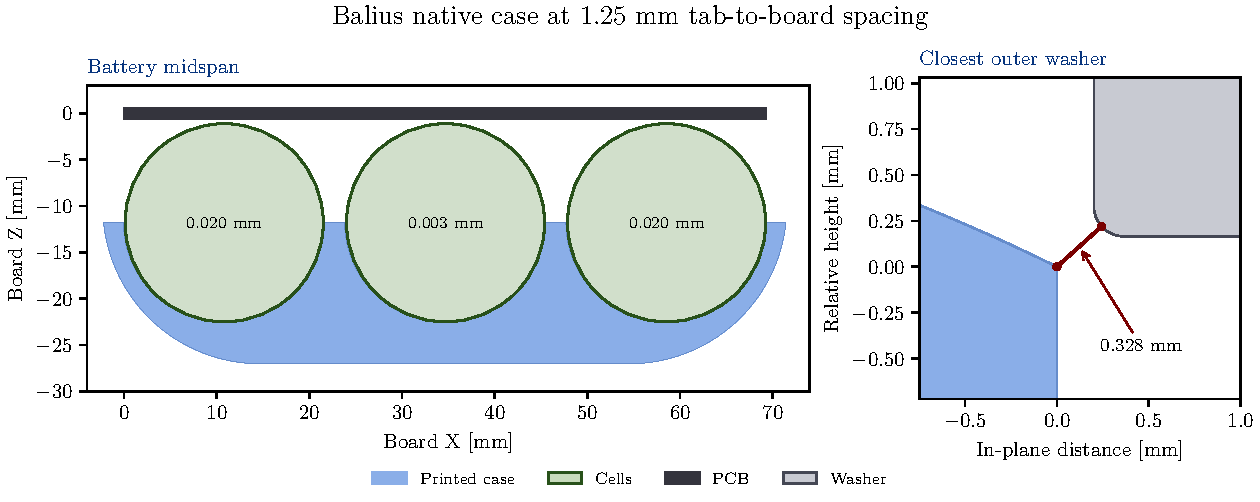
\includegraphics[width=\linewidth]{figures/balius-native-fit-1p25mm.pdf}
\captionof{figure}{The left panel cuts through the battery midspan. Each cell label gives its shortest three-dimensional distance to the case. The right panel cuts through the two closest points on the outer washer and case, using a separate magnified scale.}\end{center}

\begin{center}\small\begin{tabular}{lrr}\toprule
Assembly quantity & Bare board & Snug Balius geometry\\\midrule
Battery cells / nickel-strip attachments & 3 / 6 & 3 / 6\\
Original battery-fastener preload & $6\times750$ N & $6\times750$ N\\
Added mounting screws & 0 & 4 (nylon or aluminium)\\
Printed solid volume & 0 & 62.980 cm$^3$\\
Mass of board plus printed shell$^\ast$ & 251.82 g & 325.51 g\\\bottomrule
\end{tabular}
\captionof*{table}{$^\ast$The bare value is the archived model mass. A dense PLA shell at 1.17~g/cm$^3$ adds 73.69~g, or 29.3\%. The estimate excludes the four added screws and spacer material. Actual print mass has not been measured.}\end{center}

\heading{Mounting and contact assumptions}
The native export has 6.350~mm thick tabs at the four case screw bearings. The nominal distance from the PCB underside to each modeled screw-bearing plane is 7.600~mm. Both variants use the same hole registration and air around the cells. The added screw shanks have nominal M4 geometry. The plastic scenario uses the nylon properties from the original comparison; the metal scenario uses aluminium. The 1.25~mm spacers are represented by the same assumed printed-PLA compression law. The four added screws have no specified installation torque.

\newpage
\pageheading{Comparison baseline and native rerun}
The reference is the same no-case assembly across both screw-material comparisons. It includes the original board, all three batteries, their nickel strips, and the six preloaded fasteners. The global comparison uses the eight original mounting faces, three separate base-excitation axes, the original 20--2000~Hz spectrum and the nine-second seeded acceleration records. The edge-cell fixtures retain the earlier clamp preload, weld idealization, and nickel laws so changes in reaction or strain can be traced to the snug case.

\begin{center}\small\begin{tabular}{lr}\toprule
Verified no-case result & Value\\\midrule
Peak PCB displacement during bolt tightening & 47.46~$\mu$m\\
First connected prestressed natural frequency & 485.96 Hz\\
Peak PCB Z displacement, base Z & 52.67~$\mu$m RMS\\
Peak PCB equivalent stress, base X & 90.33 MPa RMS\\
Bilinear nickel, force at $+0.500$ / $-0.500$ mm cell travel & $+8.54$ / $-8.51$ N\\\bottomrule
\end{tabular}
\captionof*{table}{Static displacement, RMS response and prescribed-travel reactions describe different load cases.}\end{center}

\heading{Resolving the initial contact}
The 2~mm case mesh contains 45,549 quadratic tetrahedra and 77,166 nodes. Its integrated solid volume differs from CAD by 0.00089\%. A second mesh with a 3~mm size limit contains 18,051 tetrahedra. Both have positive minimum scaled Jacobians. With the finer mesh, all three undeformed cell skins remained clear at 1.250~mm at both surface sampling levels. At the higher sampling level the middle cell first reached the moving surface at 1.2412--1.2414~mm, compared with 1.2396--1.2400~mm in CAD. Coarser surface sampling on the 3~mm mesh gave an apparent initial intersection. The native contact search reported a minimum initial gap of 0.002969~mm, within 0.000037~mm of CAD. Its reported penetration tolerance was 0.196~mm. The actual penetration and force on loaded faces must be recovered at each converged bolt-tightening state.

\heading{Response quantities}
The native comparisons will report mounting reactions, board deformation, cell and washer contact, matched natural modes, signed and RMS vibration quantities, tension along and across the printed layers, and edge-cell force and nickel damage for both pull directions where supported by the fixture. The 22 movie subjects use the bare board as the reference on shared physical or display scales. The snug-fit response values will be filled from audited native outputs. Appendix~A preserves the previous study with its original geometries and page numbering.

\clearpage
\setcounter{page}{1}\renewcommand{\thepage}{A-\arabic{page}}
\setcounter{figure}{0}\renewcommand{\thefigure}{A.\arabic{figure}}
\setcounter{table}{0}\renewcommand{\thetable}{A.\arabic{table}}
\renewcommand{\theHfigure}{appendix.\arabic{figure}}\renewcommand{\theHtable}{appendix.\arabic{table}}
\fancyhead[R]{\small\color{B}Appendix A\quad Previous fit study}
\pdfbookmark[0]{Appendix A. Previous battery-case study}{prior-study}
{\LARGE\bfseries\color{B}Appendix A. Previous battery-case study}\par
{\large Assembly fit, bolt tightening, side pull and vibration response}\par
{\small 9 November 2026\quad|\quad Native structural analysis in ANSYS MAPDL 2026 R1.02\quad|\quad\href{https://github.com/MDNich/MIT-RT-26_27-Work/blob/main/simulation_work/avionics/powerboardsim/2/output/videos/README.md}{22 paired movies}}
\heading{The mounting height determines whether the cells are already loaded}
Placing the four tabs directly against the board creates approximately 1.18~mm of interference at the cell crowns. Each of the three cell solids shares about 1.70~cm$^3$ with the undeformed enclosure. A 3~mm tab stand-off clears the cells, nickel strips, washers and fasteners present in the 35-body mechanical STEP assembly. Thus a flush installation must displace or deform parts as the screws tighten. With the supplied Balius STEP, the outer washers touch at 2.397~mm stand-off. The Balius SolidWorks part has different washer clearance (page~29). Translating a rigid cell along the PCB X axis first closes a gap after 0.146--0.325~mm, depending on the cell and direction. Flexible relative motion determines whether contact occurs under load.
\begin{center}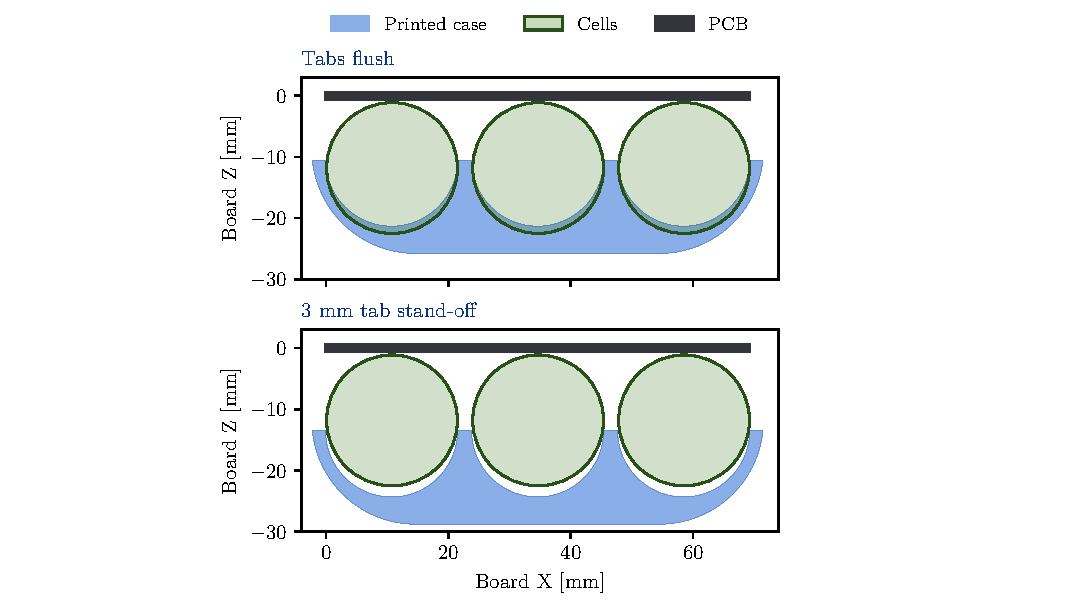
\includegraphics[width=.94\linewidth]{figures/midspan-fit.pdf}
\captionof{figure}{Section through the middle of the cells, in PCB coordinates. The solid outlines show as-designed geometry before tightening. The mounting tabs lie beyond this section.}\end{center}
\heading{What the raised case changes}
Under X-axis vibration, the 3~mm case increased peak board-normal motion from 23.37~$\mu$m RMS bare to 145.55 with nylon screws and 120.00 with aluminium. Under base Z the peak PCB stress rose from 32.5~MPa RMS bare to 64.8 with nylon and 84.2 with aluminium (page~13). With the bilinear nickel law, an 8.54~N pull moved the edge cell 0.50~mm bare and about 0.20~mm with either raised case. With the multilinear law, a fixed 0.3375~mm travel required 10.15~N bare, 63.82~N with nylon and 125.98~N with aluminium screws (page~26). Nylon also gave the lowest cell-body X acceleration. Aluminium reduced board movement relative to nylon and increased the local stress across the PLA layers at a screw bearing. In the flush mounting trials, the printed-PLA tensile reference was exceeded before the tabs touched. At the last nylon equilibrium, only 4--5\% of each tab lay within 0.05~mm of the board. With aluminium, that fraction was 18--19\% even at the full 3~mm screw travel (page~19).

\heading{Reference assembly}
The October assembly has 208 bodies and a modeled mass of 251.82~g. Eight stand-off end faces carry the base motion. Two nickel strips attach each cell to the assembly. In the connected reference, six existing screws were loaded to 750~N apiece and locked. Its first mode was 485.964~Hz. Independent base excitation between 20 and 2000~Hz gave a maximum PCB directional displacement of 0.052674~mm RMS under Z excitation and a maximum PCB equivalent stress of 90.325~MPa RMS under X excitation. These archived quantities supply reference checks for the repeats.
\newpage
\pageheading{Registration and fastener selection}
The four nonplated corner holes in PCB1 ODB++ have finished diameter 4.200~mm. The hole pattern measures $62.865\times114.427$~mm. The case bores have two diameters, 5.000 and 5.090~mm, on a $62.855\times113.241$~mm pattern. Centring the two patterns leaves about 0.593~mm of offset at each end. The sum of the radial clearances of a nominal 4~mm shank in the smaller case bore and in the board is 0.600~mm. The approximately 0.007~mm difference is the available nominal alignment margin there. Printed hole size, fastener major diameter and drilling tolerances therefore matter for installation.
\begin{center}\small\begin{tabular}{lrrr}\toprule
Tab stand-off [mm]&Cell overlap [mm$^3$/cell]&Washer bodies intersected&Other intersections\\\midrule
0&1696--1698&4&6 nickel strips\\
1.2715&0&4&None found\\
2&0&4&None found\\
3&0&0&None found\\\bottomrule\end{tabular}
\captionof{table}{Solid intersections between the unstrained case and mechanical STEP bodies. The board's lower face defines the tab seating datum.}\end{center}
Starting from 3~mm of tab stand-off, the four outer washers meet the descending case after 0.603~mm. The middle cell first touches after 1.760~mm and the two outer cells after 1.790~mm. Once a washer touches, actual motion depends on deformation of the case and fasteners. A rigid assembly at the nominal registration therefore needs more than 2.397~mm of stand-off for clearance. Manufacturing tolerances and assembly misalignment would change that value.
\begin{center}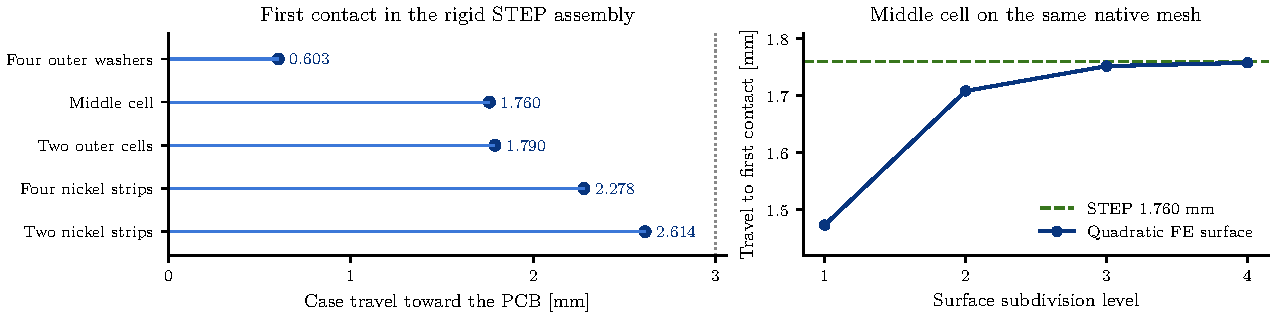
\includegraphics[width=.96\linewidth]{figures/flush-drawdown-fit.pdf}
\captionof{figure}{Left, downward travel from the 3~mm position. Solid intersections 0.05~mm beyond each onset independently confirm contact. Right, subdividing the same curved finite-element surfaces moves the middle-cell contact toward the STEP solution. The underlying case mesh and the physical geometry are fixed.}\end{center}
\heading{Materials and mounting representation}
The supplied single-solid STEP has volume 63.069~cm$^3$. At a printed-PLA reference density of 1.17~g/cm$^3$, a dense case weighs 73.79~g, about 29.3\% of the bare assembly mass. The material axes place the print layers parallel to the PCB for this scenario. PolyLite PLA coupon tensile moduli are 3.427~GPa in the print plane and 3.065~GPa through the layers. Shear moduli and Poisson ratios are engineering assumptions. Actual infill, orientation, print parameters and case mass require measurement. The published coupons used 100\% infill. \href{https://wiki.polymaker.com/polymaker-products/more-about-our-products/documents/technical-data-sheets/pla/polylite-tm-pla}{Polymaker technical data sheet.}

The candidate model uses four M4 beam shanks with an effective tensile area of 8.78~mm$^2$. The comparison uses 69~GPa for aluminium and an exploratory 3.0~GPa for nylon. The nominal nylon hardware is McMaster-Carr 93640A145, M4 $\times$ 0.7 thread, 12~mm long. The represented bearing patches transfer loads between each end and its solid mesh. Compression-only members represent tab seating, with an assumed PLA annulus at the raised attachment points. The four case screws have no measured installation torque. The 750~N in the reference applies to the six original battery fasteners. \href{https://www.mcmaster.com/products/nylon-allen-screws/}{McMaster-Carr metric socket-head screws.}
\heading{Numerical checks and remaining comparisons}
The initial mesh has 16,108 curved quadratic tetrahedra. A 43,659-element refinement is available. Both have positive minimum scaled Jacobians. The native preparation check counted four screw beams, four compression seats and 8,038 candidate case contact faces. The raised cases passed the preload checks used for their vibration comparisons. In both flush cases the PLA exceeded its tensile reference before the tabs seated (page~19). The October bare-cell damage run and its repeat first registered damage around 43~N. A physical breaking load remains undetermined.
\newpage
\pageheading{The bare-board repeat reproduces the six locked bolt loads}
The original battery attachment provides the initial stress field for the connected modal and vibration analyses. In the first nonlinear load step each of the six pretension elements receives 750~N. In the second step MAPDL holds the attained section adjustment fixed. The reaction at the pretension degree of freedom then measures how much load the locked joint retains. The four case screws are absent from this reference run.

\begin{center}\begin{tabular}{rrr}\toprule
Existing bolt & Locked adjustment [$\mu$m] & Locked reaction [N]\\\midrule
1 & 28.297 & 749.99935\\
2 & 22.205 & 749.99945\\
3 & 18.597 & 749.99908\\
4 & 30.457 & 749.99680\\
5 & 20.686 & 749.99942\\
6 & 18.772 & 749.99868\\\bottomrule
\end{tabular}
\captionof{table}{Fresh MAPDL extraction after length locking. Every row agrees with the October export at its stored precision. The largest departure from the applied 750~N is 0.00321~N.}\end{center}

The solver stored eight equilibrium states and completed the two load steps in approximately 59 minutes on 12 distributed processes. The largest total displacement at lock was 0.0474595~mm. The repeated result differs from the October Mechanical export by $3.4\times10^{-8}$ in relative terms. The model produced 45 warnings, including overlapping contacts, automatically removed redundant constraints and the fixed orientation of pretension elements during large-displacement analysis. The warning text printed in the main solver listing matched the reference run. This comparison establishes repeatability for the existing attachment. Page~7 compares the locked bare and raised assemblies. The vibration response requires separate modal and random-response results.

\heading{How the side-pull comparison measures load transfer}
The local model drives the outer cell sideways through its rigid pilot while the two nickel strips bend. In the washer-clamped fixture, each strip is compressed with 750~N and the clamp height is then locked. During the pull, the cell can translate in the other two directions and rotate. The cased fixture adds a deformable printed enclosure, four screw shanks and compression-only tab seats. The neighboring cells and screw tops are fixed in this local approximation. The native model check counted 9,502 potential PLA contact faces. These contacts carry compression between PLA and the cell or washer surfaces. Direct PLA-to-nickel contact is omitted from this local fixture. That omission matters most in the flush geometry, where the CAD also intersects the strips.

The audit sums external forces and moments about the displaced cell centre at each converged increment. Both nominal nickel studies used the same bare mesh and 750~N clamp preloads. At 0.500~mm lateral travel, the bilinear model (148~MPa initial yield) required 8.54~N, and the multilinear damage model (185~MPa initial yield) required 11.33~N. At the same 8.54~N, the refined multilinear bare and raised-nylon histories both gave 0.20190~mm between saved states at 0.20166 and 0.20215~mm. The two loading schedules used different increments. Page~6 compares enclosures using the bilinear law throughout.

With the continuous nickel-damage law, the October run and its fresh repeat reached the same 110 equilibria. Both first crossed the $10^{-4}$ damage threshold between 3.250 and 3.275~mm, at 42.87--43.37~N. The maximum force difference over the two curves was $2.5\times10^{-8}$~N. At their last converged state (3.347~mm, 44.86~N), four flat shell elements exceeded the threshold on the bottom face, two per strip, over 1.50~mm$^2$ of original shell area. The force was still rising when convergence stopped. The rupture load remains undetermined.

\begin{center}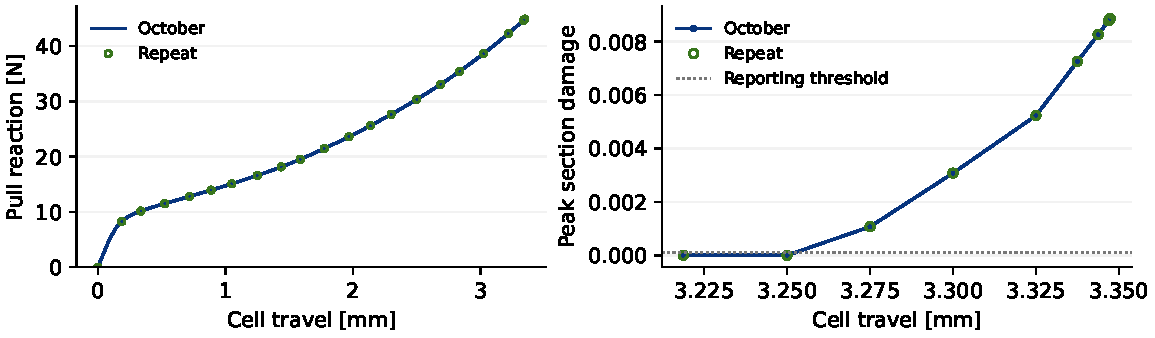
\includegraphics[width=.90\linewidth]{figures/bare-nominal-damage-repeat.pdf}
\captionof*{figure}{Native bare edge-cell pull through the last converged equilibrium. The right panel enlarges the onset interval. Damage is the largest reported shell-section value in the two strips.}\end{center}

\newpage
\pageheading{Both default-contact meshes reproduce the October modal spectra}
Each unpreloaded model used the archived mounting constraints and searched for 20 undamped natural frequencies between 1 and 10,000~Hz. The original mesh returned modes from 62.805 to 2205.547~Hz and the refined mesh from 66.611 to 2247.595~Hz. The maximum relative differences from the corresponding October exports were $1.78\times10^{-8}$ and $1.74\times10^{-9}$. Repeating a given discretization thus produced the same frequency spectrum to the stated precision.

\begin{center}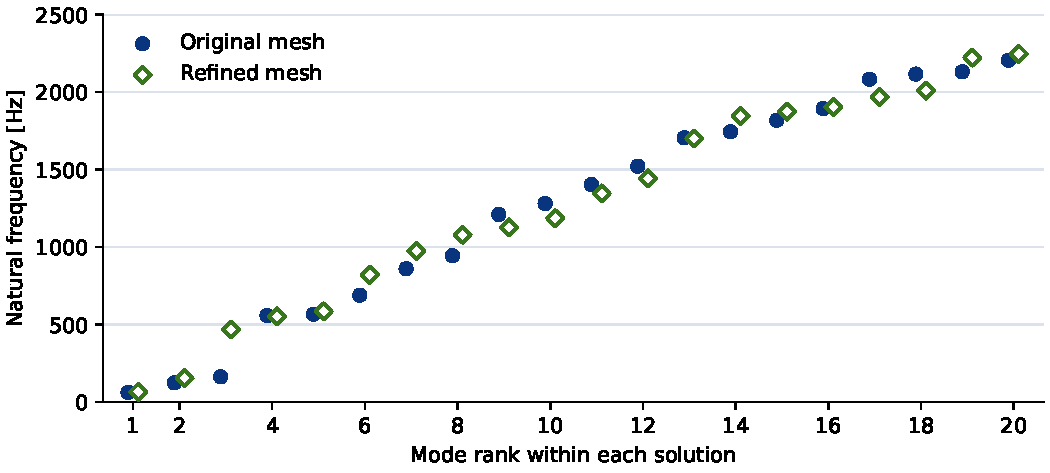
\includegraphics[width=.73\linewidth]{figures/bare-modal-frequencies.pdf}
\captionof{figure}{Fresh ANSYS results with the original default contacts. Rank orders the frequencies within each mesh. A shared rank can contain different mode shapes, particularly where modes exchange order.}\end{center}

The first original-mesh run returned only four modes and exited normally. The repeat kept the same input geometry, material properties, supports and search range. It changed the Block Lanczos algorithm to its alternate formulation and requested the Sturm sequence check. This recovered the complete spectrum. The default models retain the detached nine-body group in the earlier connection diagnosis. The bearing, locking and contact states of the six-bolt model provide the starting point for the connected vibration comparison.

\heading{PCB stress over the 480 frames of the seeded motion movie}
Each of the three 9~s October base records has 589,825 samples at 65,536~Hz. After a 0.1~s ramp, the periodic 20--2000~Hz input reaches 14.136~g RMS. The native histories used 38 prestressed modes for the bare board, 49 with raised nylon screws and 48 with raised aluminium screws. All use 2\% damping. Each clip shows 480 signed states from 1.000061 to 1.029297~s at 60 frames per second.

The six signed dynamic stress components were summed at each of 312,112 PCB element corners before calculating von Mises stress. The fresh native X history reproduced all 480 October bare-board frame maxima within 0.000028\%; the independent integration agreed within 0.00182\%. The largest native value in this clip was 154.41~MPa bare, 169.95~MPa with nylon screws and 151.03~MPa with aluminium screws. The nylon peak occurred about 3.85~ms earlier and at a different board node from the bare peak.
\begin{center}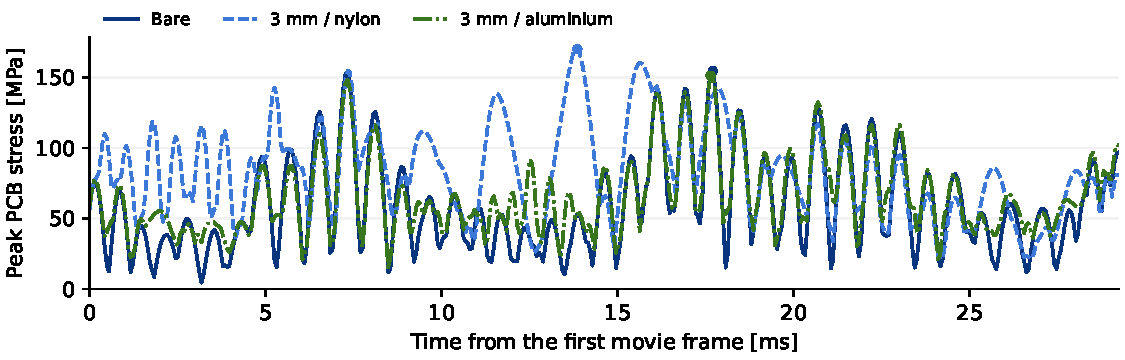
\includegraphics[width=.82\linewidth]{figures/raised-seeded-pcb-stress_native.pdf}
\captionof{figure}{Maximum dynamic PCB stress at each of the original 480 movie times. The three curves use signed native MAPDL coordinates on the corresponding tightened modal bases. Each dot marks a clip maximum.}\end{center}

Over the same frames, native peak board-normal displacements for base X/Y/Z were 0.040/0.047/0.168~mm bare, 0.244/0.154/0.290~mm with nylon and 0.114/0.125/0.314~mm with aluminium. All 22 pairs use native fields. The seven time-history pairs display motion at $50\times$ scale and $273\times$ slow motion. \href{https://github.com/MDNich/MIT-RT-26_27-Work/blob/main/simulation_work/avionics/powerboardsim/2/output/videos/README.md}{Paired movies.}
\newpage
\pageheading{Does the contact model start with the gap measured in CAD?}
An enclosure that presses on the cells at the start of a raised-case calculation will appear to stiffen the assembly before the real parts would touch. We checked the undeformed contact pairs separately from the load solution. The local fixture uses one target for the moving edge cell and another for the fixed neighboring cells and washers. The global assembly uses deformable targets. The search radius tells MAPDL which nearby facets to examine; it does not set the physical clearance.

\begin{center}\small
\begin{tabular}{p{.39\linewidth}rrr}\toprule
At 3 mm tab stand-off & Default search & 0.6 mm search & 2 mm search\\\midrule
Local: moving edge cell & $+0.212$ & $+0.212$ & $+0.212$\\
Local: fixed cells and washers & $-7.685$ & $+0.200$ & $+0.200$\\
Global: enclosure to assembly & $+0.199$ & $+0.199$ & $+0.199$\\\bottomrule
\end{tabular}
\captionof{table}{Initial native contact check in millimetres. Positive values are gaps; negative values are overlaps. Default search radii ranged from 10.6 to 11.1 mm. The 1 mm search reproduced the 0.6 and 2 mm columns.}
\end{center}

The CAD solids do not intersect at this stand-off. We rejected the first raised local calculation because its 7.685 mm overlap contradicted that independent check. It did not reach a converged load increment. The replacement uses a 1 mm search radius for the two added contact pairs and leaves the nickel clamp contacts unchanged. The comparison calls for the cell travel at first closure, contact pressure, penetration, and load transferred to the case mounts.

The shortest unloaded distance from any cell to the STEP case is 0.144--0.161~mm. Translating the edge cell rigidly along X first closes the gap at 0.163~mm in positive X and 0.308~mm in negative X. In the loaded fixture the cell also rotates and moves vertically.

\heading{The cell reaches the STEP case before the native contact pair carries load}
We recovered each cell pose from the motion of 784 nickel nodes rigidly attached to the cell. In both raised nominal damage fixtures, those motions fitted one rigid transformation to within $10^{-5}$~mm and reproduced the independently exported cell-pilot translations. A separate displacement readback covered all 29,610 printed-case nodes. At the stations below, their maximum movement was below $10^{-9}$~mm.

\begin{center}\small\begin{tabular}{lccc}\toprule
Cell travel & STEP solids & Meshed contact faces & Native contact reaction\\\midrule
0.1375~mm & 0.02583~mm gap & Disjoint & 0~N\\
0.1875~mm & 0.1183~mm$^3$ overlap & Intersecting & 0~N\\
0.211914~mm & 0.4864~mm$^3$ overlap & Intersecting & 0~N\\\bottomrule
\end{tabular}
\captionof*{table}{Both screw materials gave all three rows. The final row is the last open state of each refined pull. Independent intersection tests used the actual cell target facets and only the PLA faces selected for contact. Both surface refinements gave the same classification.}\end{center}

At 0.1875~mm the cell was 23.4--23.6~$\mu$m past first STEP contact along X with its rotation and transverse translations held at their measured values. At the final open station for either screw material this excess travel reached 47.8--48.0~$\mu$m. Testing only the target vertices missed intersections between faces at 0.1875~mm. The finer load steps on page~25 resolve when this model carries force. Contact discretization also affects how that force relates to the physical assembly.

\heading{Why the flush installation needs a separate check}
The flush STEP has real interference. In the local model, a 2 mm search recovered the 1.178 mm crown overlap of the moving cell. A 1 mm search found only 1.000 mm, and a 0.6 mm search found only 0.598 mm. Tightening the search around the flush configuration can therefore hide real interference. Conversely, the default global search reported a peak overlap of 10.093 mm, versus 1.848 mm with a 2 mm search. These values identify a contact-model discrepancy. They do not establish an installation force. The flush comparison requires a verified path into contact, including the washers and strips, and force balance in the installed assembly before the vibration solve.
\newpage
\pageheading{Both raised cases restrain the edge cell after contact}
The local fixture pulls the outer cell in positive X. Its other translations and rotations are free. With the case on a 3~mm stand-off, the last open state was at 0.196~mm and the first closed state at 0.221~mm for either screw material. Under the 8.54~N load that moved the bare cell 0.50~mm, both cased cells travelled about 0.20~mm. The interpolated estimates were 0.207~mm with nylon and 0.202~mm with aluminium. Both lie in the same 0.025~mm interval between native states.

\begin{center}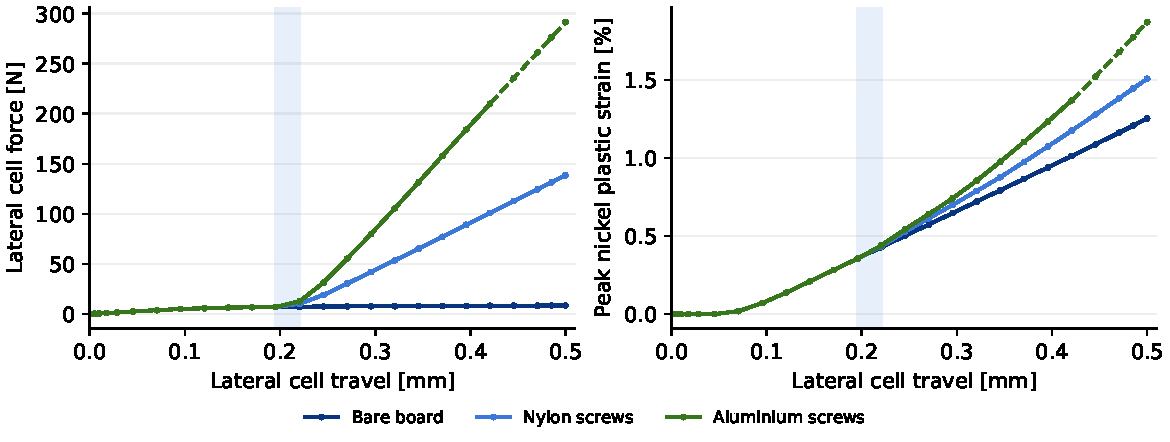
\includegraphics[width=.94\linewidth]{figures/raised-pull-comparison.pdf}
\captionof{figure}{All three native pull histories. The blue band brackets first contact. The dashed aluminium segment extends from the last state below both PLA tensile references to states above at least one reference.}\end{center}

\begin{center}\small\begin{tabular}{lrrr}\toprule
At 0.420625 mm prescribed cell travel & Bare & Raised nylon & Raised aluminium\\\midrule
Cell reaction in X [N] &8.26&100.99&209.96\\
Load on four case supports in X [N] &---&80.00&174.54\\
Peak equivalent plastic strain in nickel [\%] &1.013&1.176&1.370\\
External work applied to cell [mJ] &2.63&11.91&22.56\\
Energy stored in printed case [mJ] &---&5.41&12.93\\
Energy stored in four screw shanks [mJ] &---&2.05&2.61\\\bottomrule
\end{tabular}\end{center}

At a fixed travel the stiffer aluminium attachment increased both the case load and the strain in the nickel. At a fixed 8.54~N, the native states bracketing that force instead gave 0.36--0.44\% peak nickel plastic strain for the two cased curves, versus 1.25\% bare. Integrating native nodal forces and moments over the displacements of the PLA and shanks independently reproduced their stored energies within 0.009\% of each component's maximum change.

\heading{Where the aluminium comparison leaves the coupon range}
With aluminium screws, peak in-plane PLA tension crossed 52.3~MPa between 0.421 and 0.446~mm. Through-layer tension crossed 40.5~MPa between 0.446 and 0.471~mm. Both peaks were within 0.54~mm of the idealized screw bearing. At 0.50~mm the elastic continuation returned 291.5~N with aluminium, versus 138.5~N with nylon and 8.54~N bare. The nylon case stayed below both references, reaching 28.6 and 23.5~MPa. Its most tensile shank fibre reached 30.5~MPa, including 29.3~MPa from bending.

All fixtures saved 33 converged states. Peak penetration at a loaded cell/case corner was 0.0116~mm with nylon and 0.0198~mm with aluminium. The native cell contact forces and case-support reactions balanced to within 0.0019~N. These pulls assume fixed screw tops and omit direct PLA-to-nickel contact. At 0.421~mm cell travel, the axial-load resultants at the four tab bearings acted 5.41--6.54~mm from the screw axes with nylon and 5.41--5.49~mm with aluminium. All eight offsets exceed the modeled 3.75~mm bearing radius. A one-sided axial pressure across that footprint cannot carry the same force and moment. The computed pull stiffness therefore depends on how the installed joints transmit a couple. Page~17 gives the force check.

\newpage
\pageheading{Both raised cases reduce board deflection during tightening}
The bare board and both 3~mm stand-off assemblies completed eight equilibrium states under the same six-bolt tightening sequence. Each original bolt carried 750~N before its length was locked and retained 749.996--750.000~N afterward. The two cased models differ only in the properties assigned to the four case screws. The load in this comparison comes from the six original bolts.

\begin{center}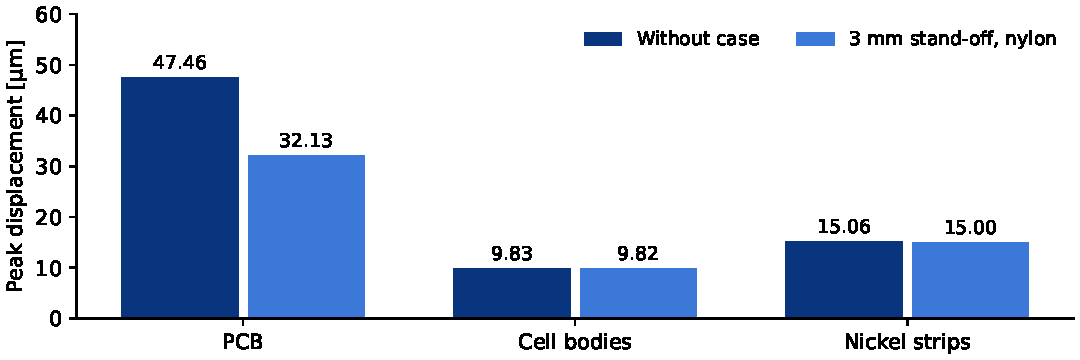
\includegraphics[width=.93\linewidth]{figures/raised-static-comparison.pdf}
\captionof{figure}{Peak displacement magnitude relative to the undeformed assembly after bolt locking. Each comparison uses the same mesh nodes on each part. Micrometres are used here to show the small changes at the cells and nickel strips.}\end{center}

The peak PCB displacement occurred at node 207485 in all three models. It fell from 47.46~$\mu$m bare to 32.13~$\mu$m with nylon screws and 27.13~$\mu$m with aluminium screws, reductions of 32.3\% and 42.8\%. Changing the four case screws from nylon to aluminium reduced this peak by another 5.00~$\mu$m, or 15.6\% relative to nylon. The cell-body peak changed by at most 0.30\% from bare and the nickel-strip peak by 0.51\%. All 8,038 case-to-assembly contact faces stayed open in both raised assemblies, with zero contact pressure at every stored state. The case altered board bending through its four corner attachments.

ANSYS DPF recovered translations on 217,704 common PCB nodes. On the bare control the two displacement readers agreed on every component. The six pretension adjustments agreed with native MAPDL readback within $10^{-11}$~m in all three assemblies.

\heading{The PCB bends toward the cells in both flush installations}
The PCB moved less than 1~$\mu$m through 0.50~mm screw travel. At 0.80~mm, after washer contact, the same corner at $(0,0)$ had moved 0.197~mm toward the cells with nylon screws and 0.216~mm with aluminium. The aluminium screws raised the total drive force by 44\% and peak board motion by 9.6\%. The four PCB bearings moved 0.104--0.145~mm with nylon and 0.125--0.163~mm with aluminium.

\begin{center}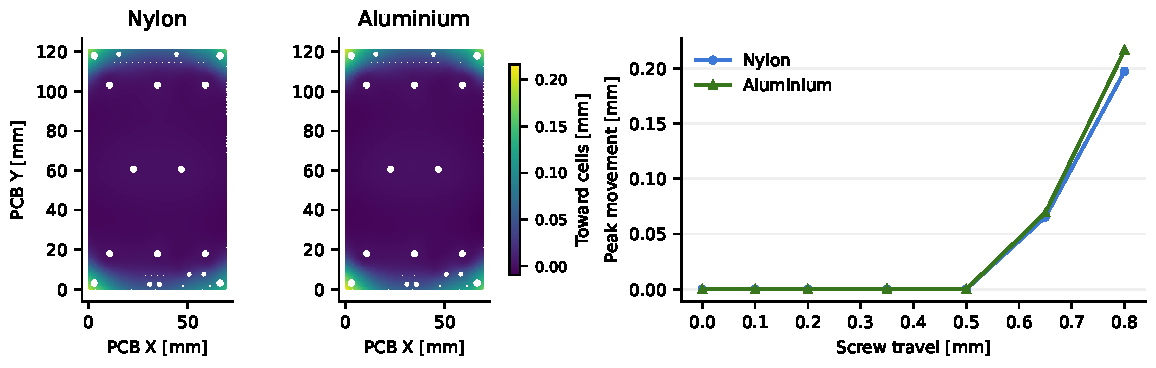
\includegraphics[width=.96\linewidth]{figures/flush-pcb-screw-comparison.pdf}
\captionof*{figure}{Upper PCB face at 0.80~mm screw travel, with one displacement scale for both maps. Positive movement is toward the cells. The curves show the maximum across all 217,704 board nodes relative to six-bolt lock. }\end{center}

At 0.80~mm, the largest increase in upper-face principal tensile strain from six-bolt lock was 0.601\% with nylon and 0.958\% with aluminium. We compared the same element corner before and after driving. Excluding points within 2~mm of a tied PCB bearing node gave 0.601\% and 0.670\%, respectively. These local elastic strains describe the board laminate model.

\newpage
\pageheading{The raised enclosure adds resonances below the first bare-board mode}
We extracted undamped natural frequencies about the verified bolt-locked states, using the same mounting constraints and a 1--4000~Hz search. The assembled masses were 251.82~g bare, 325.82~g with the raised nylon-screw case and 326.10~g with aluminium screws. The models returned 38, 49 and 48 modes, respectively. The lowest three frequencies were 253, 289 and 339~Hz with nylon and 320, 372 and 378~Hz with aluminium. All six fall below the first bare-board mode at 486~Hz.

\begin{center}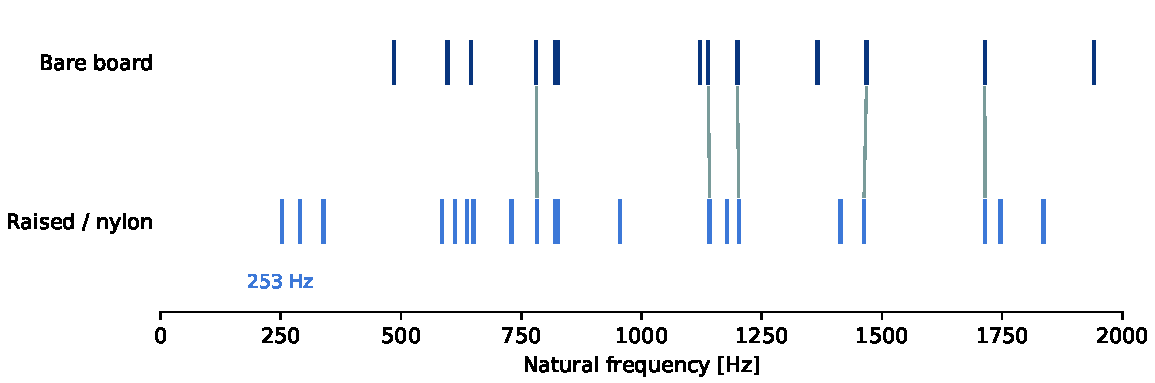
\includegraphics[width=.96\linewidth]{figures/raised-prestressed-modes.pdf}
\captionof{figure}{Each tick marks one native frequency in the excitation band. Lines connect five bare-to-nylon matches above MAC 0.94, and nylon-to-aluminium matches above MAC 0.97 where the assigned match is also the best available match.}\end{center}

The 253~Hz mode carried 17.9\% of the assembled mass in X translation. In this shape the largest cell displacement was 2.8\% of the peak on the PCB, while the peak on the case was 126\% of the PCB peak. Those are amplitude ratios \emph{within a mode}; the actual vibration displacement requires a forcing spectrum and damping. The 253~Hz mode had no close counterpart in the bare set: its highest shape correlation was 0.56. Conversely, the bare 781.35~Hz mode matched cased mode 9 at 782.88~Hz (correlation 0.943). This battery-motion mode shifted by only 0.20\% even though its rank changed from fourth to ninth.

\begin{center}\small\begin{tabular}{lrrr}\toprule
Effective translational mass, fraction of whole assembly & X & Y & Z\\\midrule
Bare, all 38 retained modes & 87.2\% & 89.0\% & 89.6\%\\
Raised nylon, all 49 retained modes & 90.1\% & 91.5\% & 90.8\%\\
Raised aluminium, all 48 retained modes & 90.1\% & 91.4\% & 90.3\%\\\bottomrule
\end{tabular}\end{center}

\heading{How the shape comparison was made}
Both modal meshes contain their assembly's static deformation. Before comparing vectors, we checked every original solid node against its own preload displacement and matched the 369,584 node IDs and their undeformed coordinates. The modal assurance criterion (MAC) is the squared, unweighted correlation of the global X, Y and Z eigenvector components at these nodes. It ranges from zero to one and is independent of the sign and normalization of a mode. It excludes the new case nodes so that both vectors describe the same structure. Modes with weak or competing matches remain ambiguous. For the two screw materials we also matched all 399,194 solid nodes, including 29,610 PLA nodes. The first mode rose by 26.5\% from 253.16 to 320.17~Hz with full-solid MAC 0.989 and PLA-only MAC 0.994. It is a closely corresponding shape. The next two matches had full-solid MACs of 0.739 and 0.785.

The October bolted movie shows mode 20 at 2364.18~Hz. The two raised assemblies have mode 20 at 1836.45 and 1950.27~Hz. Its MAC with the bare mode is below 0.00023 in both. Searching the full native bases instead places the closest shape at mode 27, at 2365.06~Hz with nylon (MAC 0.717) and 2368.47~Hz with aluminium (MAC 0.640). The movie preserves the original rank and identifies this match on screen.
\newpage
\pageheading{The linear model predicts more PCB motion with the raised case}
We applied the October base acceleration spectrum separately along X, Y and Z to the three bolt-locked assemblies. For the 3~mm stand-off with nylon screws, the independent calculation predicts greater out-of-plane PCB motion for all three excitation directions. Under X excitation the peak PCB response in Z rises from 23.37 to 145.55~$\mu$m RMS, a factor of 6.23. In the same calculation the largest cell response in X falls from 61.43 to 53.79~$\mu$m RMS (12.4\%). With aluminium screws, the peak PCB Z responses were 120.00, 82.33 and 100.55~$\mu$m RMS for base X, Y and Z. Compared with nylon, these fall by 17.6\%, 5.0\% and 23.6\%. In particular, the 32\% reduction in static board deflection during tightening did not carry over to this vibration metric.

\begin{center}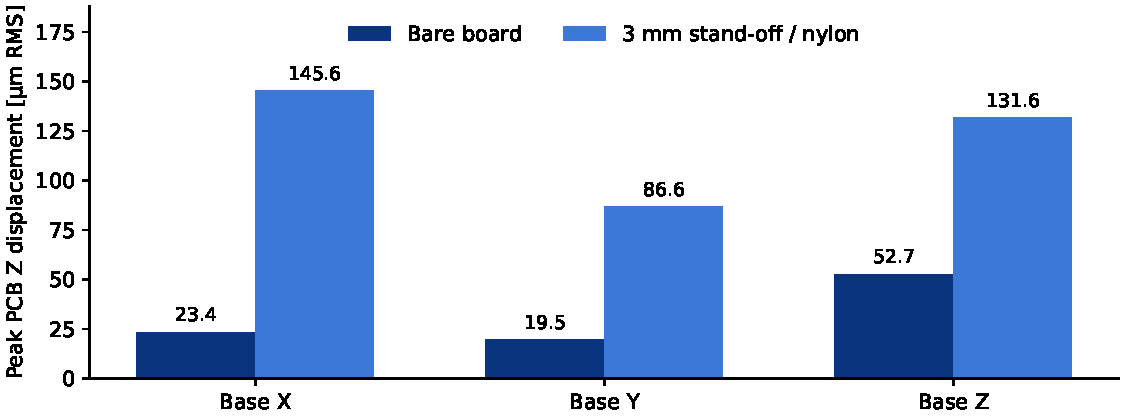
\includegraphics[width=.97\linewidth]{figures/raised-independent-psd.pdf}
\captionof{figure}{Each group compares the largest board-normal RMS displacement anywhere on the PCB under the same single-axis base spectrum. Peaks can occur at different nodes. Values describe motion relative to the supports.}\end{center}

\heading{How we checked the response}
The independent calculation uses each native mode's signed displacement field and directional participation factor. We integrate the modal frequency responses against the one-sided acceleration spectrum (20--2000~Hz, 14.14~g RMS, 2\% modal damping), including cross terms between modes driven by the same base input. This preserves cancellation and reinforcement. Halving the quadrature spacing from 0.25 to 0.125~Hz changed the modal covariance by less than $6\times10^{-8}$ in relative norm. For the bare assembly we compared all 18 peak directional displacements: three base directions, three response components, and both whole-assembly and PCB scopes. The worst difference from October's native ANSYS random-response output was 0.013\%. The three native MAPDL repeats reproduced all 51 October Mechanical maxima within $4.75\times10^{-8}$ relative, including displacement, absolute acceleration, equivalent stress and the three normal elastic strains on the PCB. Peak PCB equivalent stresses under base X, Y and Z were 90.325, 17.850 and 32.482~MPa RMS.

We repeated the independent integration with modal cutoffs of 2000, 3000, 3500 and 4000~Hz, keeping the input spectrum fixed. For the raised nylon case under base X, both the 20-mode and 49-mode calculations gave a peak PCB Z displacement of 145.55~$\mu$m RMS. Across all three inputs, increasing the cutoff from 3500 to 4000~Hz changed the nine PCB directional peaks by at most 0.22\% bare and 0.056\% cased. The bare PCB's Y response to base Y differed by 8.32\% with the 2000~Hz cutoff. These checks apply to displacement within the available basis.

The two native base-X solutions independently gave 120.00~$\mu$m for the raised aluminium case and 145.55~$\mu$m for the raised nylon assembly's peak PCB Z displacement. All 30 directional displacement peaks across five part selections per cased model agreed with the independent integrals within 0.0017\%. Both calculations linearize about the tightened contact state.

\newpage
\pageheading{The 3 mm stand-off does not prevent dynamic cell contact in the model}
The tab stand-off is not the air gap at the cells. The smallest sampled cell clearance on the tightened mesh was 0.143~mm. We paired nearby opposing surfaces and calculated their simultaneous relative motion along the local separation direction. Under base X the most exposed cell location had 0.145~mm clearance and 0.098~mm RMS relative motion. The gap there is only 1.47 times that RMS displacement. This ratio suggests contact is plausible, but it does not tell us when contact occurs.

\begin{center}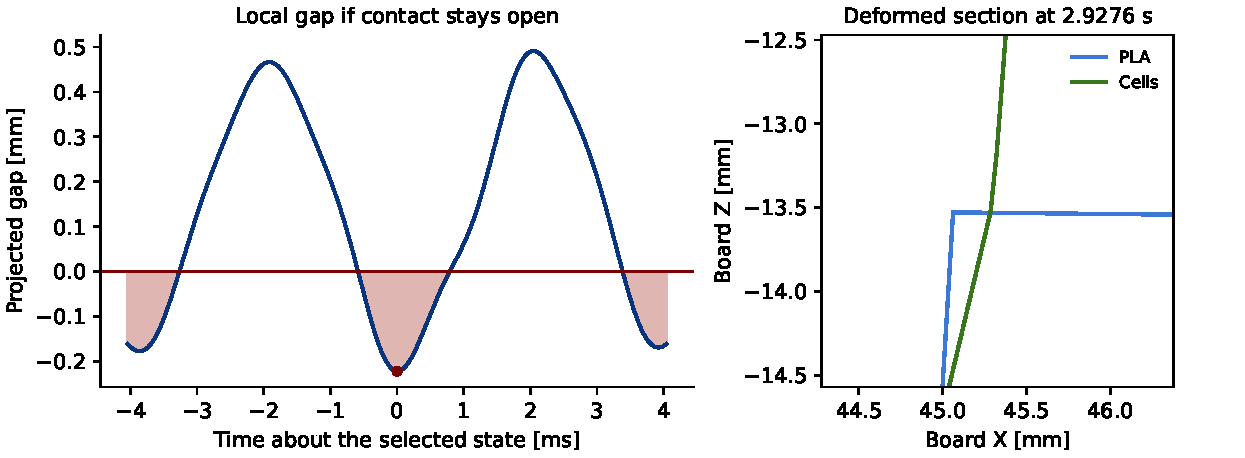
\includegraphics[width=.98\linewidth]{figures/stand3_nylon-linear-clearance.pdf}
\captionof{figure}{Raised case, nylon screws, October X-axis waveform. Left: first-order gap of the selected pair. A negative value indicates that the linear solution continues past projected contact. Right: actual-scale section of both triangulated surfaces displaced by the same signed modes. The curves are a diagnostic of the fixed-open model.}\end{center}

We independently integrated the nine-second October acceleration history and reconstructed the two skins at the instant of greatest projected approach for this pair, 2.9276~s into the waveform. At the tightened rest position the cell and case meshes had no intersections. In the selected deformed state, 895 triangle pairs intersected, and a separate signed-distance calculation placed 24 cell vertices more than 1~$\mu$m inside the PLA skin. The deepest sampled vertex lay 0.214~mm inside the PLA. Subdividing the curved elements twice more gave 0.215~mm at the same instant. Both surfaces had positive clearance before excitation. Their intersection shows where the fixed-open vibration assumption breaks down.

\begin{center}\small\begin{tabular}{lrrr}\toprule
Excitation & Cell pair gap [mm] & Relative RMS [mm] & Intersecting cell/PLA pairs\\\midrule
Base X & 0.145 & 0.098 & 895\\
Base Y & 0.143 & 0.019 & 0\\
Base Z & 0.236 & 0.112 & 0\\\bottomrule
\end{tabular}
\captionof{table}{Each row selects the cell pair with the greatest RMS-to-gap ratio for that excitation, then checks the whole cell and case skins at one instant. A zero count at one instant does not establish separation throughout the record.}\end{center}

The surface search used both centroids and vertices of facing triangles within 1.2~mm in both directions, including the midside nodes of curved elements. Under base Z the nearest-line projection became negative, but the cell and case skins did not intersect at the selected instant. Tangential motion matters: a negative projected gap alone is insufficient evidence. Under base X both independent geometric checks found overlap. Until a nonlinear transient calculation or vibration test measures the response after closure, use the preceding fixed-contact RMS results as a comparison of the two linear models, not an installed flight stress, impact load or clearance margin.
\newpage
\pageheading{The local flush installation stopped before the tabs seated}
Four nylon screws drew the printed case toward a rigid board datum from an initial 3~mm stand-off. The existing washer clamps were tightened first. ANSYS saved 88 converged equilibria before the third load step failed at the next increment. The final converged screw-head travel was 2.8685~mm, leaving 0.1315~mm of the commanded travel. The solver never reached the sideways pull.

\begin{center}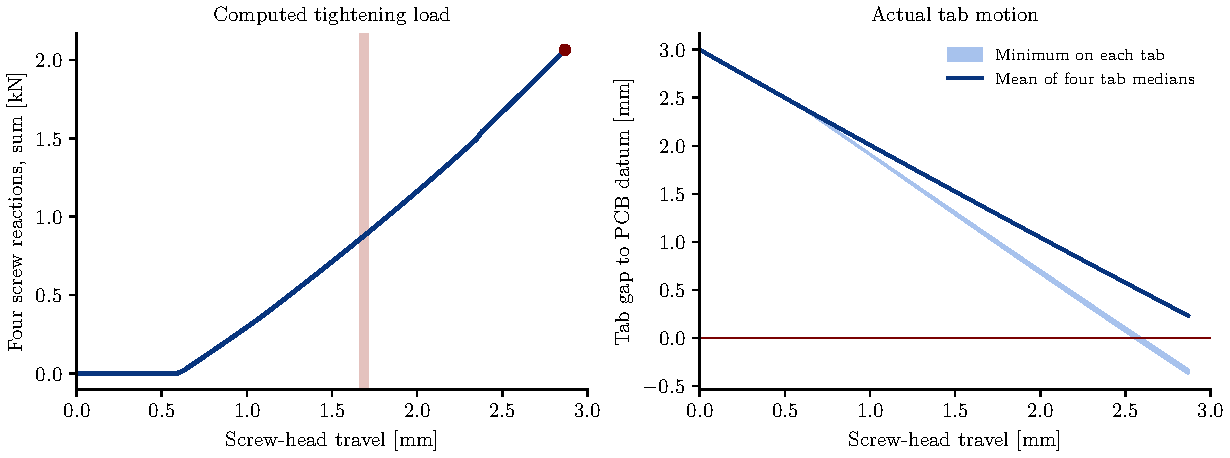
\includegraphics[width=.98\linewidth]{figures/flush-nylon-installation.pdf}
\captionof{figure}{Left, the computed total screw reaction rose to 2.066~kN. The shaded interval marks the first exceedance of the 0.05~mm numerical penetration screen. Right, the tab surfaces tilted during drawdown. At the last equilibrium every tab crossed the nominal PCB plane at some points and remained clear at others.}\end{center}

\begin{minipage}[c]{.48\linewidth}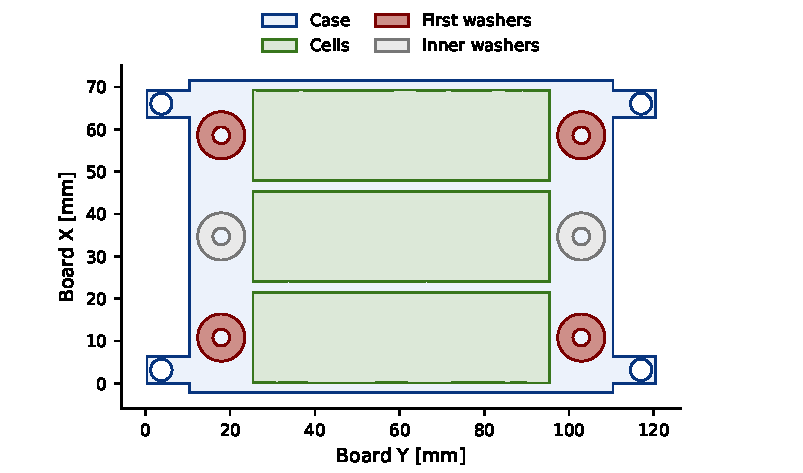
\includegraphics[width=\linewidth]{figures/washer-location.pdf}\end{minipage}\hfill
\begin{minipage}[c]{.49\linewidth}
The native fixture first loaded the four outer washers at 0.59--0.63~mm of screw travel. This brackets the independent STEP result of 0.603~mm (page~2). At 0.63~mm, two closed contact facets at each washer carried 4.89--4.92~N in board Z, totalling 19.63~N. Each loaded node lay within 0.8~$\mu$m of its assigned washer. The next nearest candidate was over 8.6~mm farther away. These local reactions apply to the fixture with fixed neighboring hardware.
\end{minipage}

The moving edge cell and its two nickel strips stayed clear throughout the partial path. Loaded-corner penetration first exceeded 0.05~mm at 1.67--1.71~mm travel and reached 0.119~mm. The largest departure from force balance was 0.030~N.

\begin{center}\small\begin{tabular}{lrrrr}\toprule
Final saved equilibrium & Tab 1 & Tab 2 & Tab 3 & Tab 4\\\midrule
Screw-head reaction [N] & 484 & 517 & 530 & 536\\
Minimum gap to board datum [mm] & $-0.332$ & $-0.357$ & $-0.366$ & $-0.369$\\
Median sampled gap [mm] & 0.248 & 0.227 & 0.236 & 0.214\\\bottomrule
\end{tabular}\end{center}

In this local fixture the seating springs moved with the screw grips, allowing a tilted tab to cross the board plane. The peak computed PLA equivalent stress reached 233~MPa under the elastic print model. The physical installation force, failure sequence, and full-flush side-pull response remain unresolved. The whole-board installation model instead places contact directly between each tab and the flexible PCB surface, so the model can develop a normal reaction at the bearing land.
\newpage
\pageheading{Contact deflects the raised case along the middle cell}
The fixed-open calculation on page~10 placed parts of all three cell surfaces inside the enclosure at the selected X-waveform sample. Along the middle cell, the affected PLA facets extended from 25.2 to 95.6~mm in board Y. We therefore retained the whole length of this contact region in two native submodels. Their outer boundaries lay 9 or 15~mm from the middle-cell contact line. Each retained the original quadratic elements and directional PLA properties.

For each domain we imposed the tightened board displacements, then applied the signed motion at 2.9276~s to the two local cell bodies and the outer cut faces of the PLA. We increased the imposed motion from zero to its full value and unloaded in a series of static equilibria. With cell contact disabled, the free PLA nodes followed the parent solution to within 1~$\mu$m. With frictionless contact active, the largest change in their motion was 249~$\mu$m in the smaller domain and 244~$\mu$m in the larger one.

\begin{center}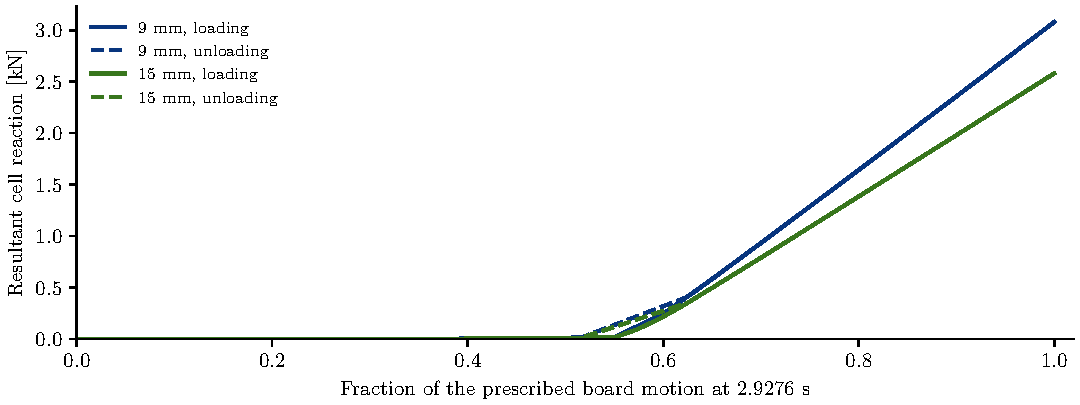
\includegraphics[width=.86\linewidth]{figures/raised-nylon-contact-replay.pdf}
\captionof{figure}{Each curve gives the force needed to impose this particular displacement path. The larger domain leaves a wider section of PLA free to flex. The peak reaction fell by 16.2\%. The local models hold the cell motion fixed as the case pushes back.}\end{center}

\begin{center}\small\begin{tabular}{lrr}\toprule
At the fully imposed displacement & 9~mm domain & 15~mm domain\\\midrule
Resultant cell reaction [kN] & 3.079 & 2.581\\
Active contact faces & 24 & 24\\
Active faces touching the artificial cut & 0 & 0\\
Maximum sampled skin overlap, contact disabled [mm] & 0.2165 & 0.2164\\
Maximum sampled skin overlap, contact enabled [mm] & 0.0424 & 0.0445\\\bottomrule
\end{tabular}\end{center}

The independent geometry check measured signed distances on vertices and facet centres inside a common 8~mm band. Some tessellated surfaces still intersected even though the largest loaded-corner penetration recorded by ANSYS was below 0.5~$\mu$m at this state. Changing the cut size changed the force appreciably despite whole-model force imbalances below 0.004~N. These results establish local deflection under imposed motion. A flight impact load requires the cells and the surrounding board to respond to contact together.

\heading{Which cell first reaches the case in the transient window?}
Using the native X history from rest, we checked every integration sample through 89.478~ms on all three curved cell skins. The centre cell was clear at 85.327~ms and intersected the case at 85.342~ms. The left cell first intersected at 85.388~ms. The right cell remained clear through the window. Both local domains captured the two intervals of centre-cell overlap. The left cell lies outside both domains, so the local reactions describe only part of the assembly load path.

At the prescribed time stations, the sealed transient inputs reproduced native translations at all driven nodes within 0.0022~$\mu$m. Between stations, linear interpolation in the 9~mm domain differed from the native motion by up to 1.04~$\mu$m with a 61.04~$\mu$s table interval and 0.26~$\mu$m with a 30.52~$\mu$s interval. These checks quantify the motion imposed on the submodels. The force curves above are from the static loading and unloading calculation.

\newpage
\pageheading{The raised case increases PCB stress under Y and Z excitation}
The native MAPDL comparison used the same X-axis base spectrum and 2\% damping on both assemblies. Each original board bolt had already been tightened and locked. With four nylon case screws at the 3~mm stand-off, the peak PCB equivalent stress fell by 1.6\%, from 90.325 to 88.847~MPa RMS. Its location moved about 54~mm across the board. The PCB's maximum normal strains in X and Y both increased.

\begin{center}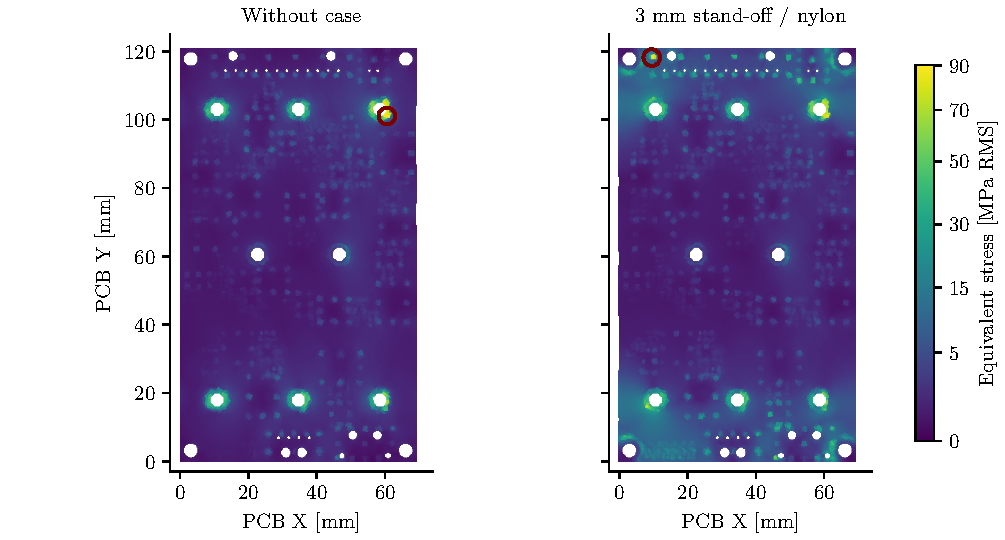
\includegraphics[width=.86\linewidth]{figures/stand3_nylon-native-x-pcb.pdf}
\captionof{figure}{PCB plan view in the original mesh coordinates. Each solid footprint shows its largest stored equivalent-stress RMS among its corners. Higher values are drawn last through the thickness. Red circles mark the maxima at $(60.55,101.11)$ and $(9.54,118.21)$~mm. Both maps use the same colour scale.}\end{center}

\begin{center}\small\begin{tabular}{llrrr}\toprule
Peak response, one sigma & Base axis & Bare & 3 mm nylon & 3 mm aluminium\\\midrule
PCB Z displacement [$\mu$m] & X & 23.37 & 145.55 & 120.00\\
 & Y & 19.45 & 86.65 & 82.33\\
 & Z & 52.67 & 131.64 & 100.56\\\midrule
PCB equivalent stress [MPa] & X & 90.32 & 88.85 & 88.65\\
 & Y & 17.85 & 57.05 & 50.29\\
 & Z & 32.48 & 64.77 & 84.19\\\midrule
Nickel equivalent stress [MPa] & X & 291.90 & 256.24 & 286.46\\
 & Y & 15.11 & 21.85 & 21.86\\
 & Z & 38.13 & 38.38 & 38.20\\\bottomrule
\end{tabular}\end{center}

Under base Z, aluminium screws gave less board travel than nylon screws and higher peak PCB stress. Each entry is a maximum over the named part. The spectra hold the tightened contact state fixed (pages~10 and~12).

An independent sum of the signed modal stresses reproduced all nine native stress-peak locations across 312,112 PCB element corners. Reducing the modal cutoff from 4 to 3.5~kHz changed the nine peak values by at most 0.20\%. With only the modes below 2~kHz, the bare base-Y peak was 34.65\% lower. The excitation band remained 20--2000~Hz throughout.

\newpage
\pageheading{The printed tab carries a local load across its layers}
The printed case and PCB react differently to the choice of screw. At the 3~mm stand-off, changing nylon screws to aluminium reduced peak PCB movement during tightening (page~7), while the greatest tensile stress normal to the layers anywhere in the PLA rose from 0.688 to 1.515~MPa. The independent orthotropic elastic-law check reproduced the stored tightening strains to within $4.0\times10^{-8}$ relative field norm across all 64,432 element corners.

For X-axis vibration with nylon screws, the native peak layer-normal stress was 17.16~MPa RMS, 0.53~mm from the nearest node tied to a screw bearing. Among corners at least 2~mm from those nodes it was 5.72~MPa RMS. The static tension at the corner of greatest RMS was 0.688~MPa. The six native component fields and stored equivalent-stress RMS agreed with integration of the signed modal stresses to within 0.001\% relative field norm.

\begin{center}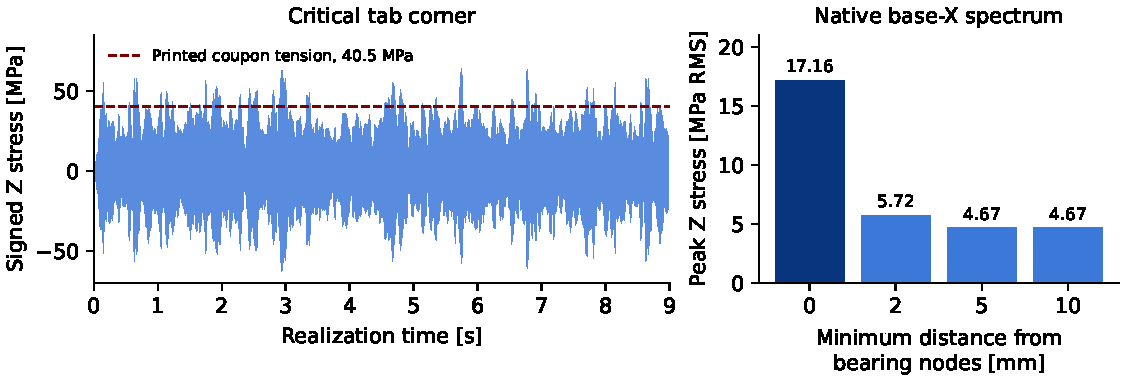
\includegraphics[width=.98\linewidth]{figures/raised-nylon-layer-stress.pdf}
\captionof{figure}{Left, independent reconstruction at element 1215221, node 815413, with the static tension included. The band preserves sample maxima and minima in 20~ms windows. Right, maximum stored through-layer RMS over locations at or beyond each distance from a coupled screw-bearing node.}\end{center}

\heading{Cell clearance at the peak printed-layer stress}
The native nine-second histories gave peak layer-normal tension above the printed-coupon mean of 40.5~MPa under all three base inputs. The table uses the corner of highest layer-normal RMS for each input and includes the locked preload. All three cell skins intersected the case at the X stress peak. At the Y and Z stress peaks, the curved skins were disjoint. These selected instants describe a linear model with fixed contact.

\begin{center}\small
\begin{tabular}{lrrrrrr}\toprule
Base & Peak [MPa] & Coupon [\%] & Time [s] & Left gap [mm] & Centre gap [mm] & Right gap [mm]\\\midrule
X & 64.3 & 159 & 5.74146 & $-0.201$ & $-0.186$ & $-0.123$\\
Y & 44.0 & 109 & 5.18582 & 0.128 & 0.111 & 0.133\\
Z & 56.2 & 139 & 7.76979 & 0.121 & 0.132 & 0.114\\\bottomrule
\end{tabular}
\captionof*{table}{Raised nylon mount. Each gap is the minimum signed distance sampled on that cell's skin at the stress peak, with eight segments per quadratic edge. Negative gaps indicate overlap. The surface-intersection check agreed at two refinements.}\end{center}

Over 589,825 samples per axis, the native modal coordinates agreed with independent integration to within 0.0015\% in relative norm. The attachment-force histories agreed within 0.0005~N over the X movie clip. The material reference comes from the \href{https://wiki.polymaker.com/polymaker-products/more-about-our-products/documents/technical-data-sheets/pla/polylite-tm-pla}{PolyLite PLA coupon data}. Actual print orientation, infill, bearing compliance and impact response remain unmeasured, so the table cannot establish whether the physical tabs crack.

\newpage
\pageheading{Aluminium screws reduce board motion and concentrate load in the tab}
The two raised models differ only in the properties of the four case screws. Both native base-X spectra used the same excitation, printed case and board mesh. Relative to nylon, aluminium reduced the peak PCB Z displacement by 17.6\% and the PCB Z acceleration by 18.6\%. The two PCB equivalent-stress peaks were within 0.22\% of each other. Changing to aluminium moved the peak back to the same node as the bare reference.

\begin{center}\small\begin{tabular}{lrrr}\toprule
Native base-X response, RMS & Bare & Raised nylon & Raised aluminium\\\midrule
PCB Z displacement [$\mu$m] &23.37 &145.55 &120.00\\
PCB Z acceleration [$g$] &52.29 &67.45 &54.92\\
Cell-body X acceleration [$g$] &103.51 &91.81 &100.90\\
PCB equivalent stress [MPa] &90.325 &88.847 &88.655\\
PLA layer-normal stress [MPa] &--- &17.16 &24.78\\
PLA layer-normal stress, at least 2 mm from bearings [MPa] &--- &5.72 &5.41\\\bottomrule
\end{tabular}\end{center}

The aluminium case had a peak layer-normal stress of 24.78~MPa RMS at a corner 0.50~mm from a coupled bearing node. That is 44.4\% above the nylon peak. Among corners at least 2~mm away, aluminium gave a slightly lower peak. This dependence on the bearing region motivates the finer case mesh and inspection of how the actual screw head bears on the print.

\begin{center}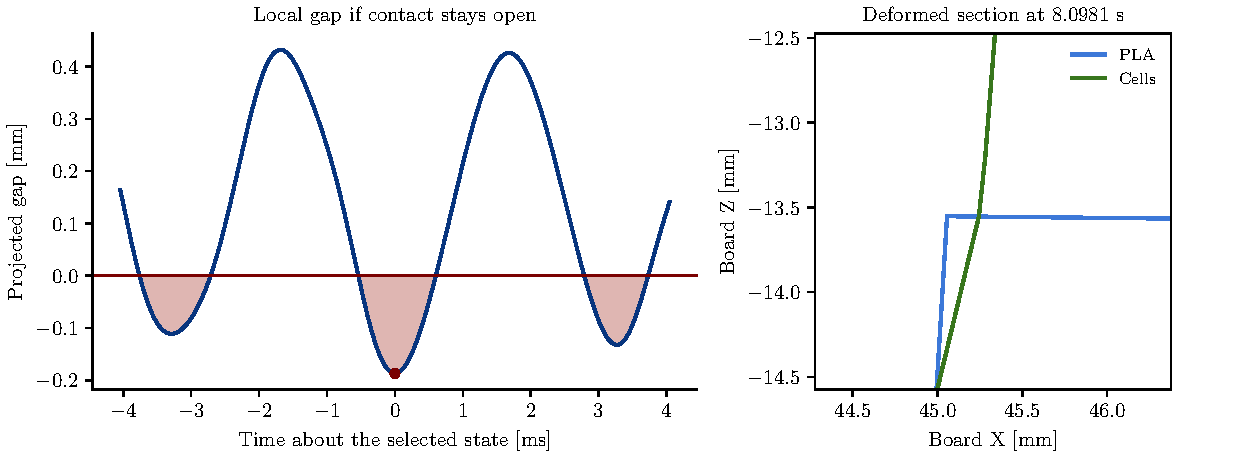
\includegraphics[width=.96\linewidth]{figures/stand3_aluminium-linear-clearance.pdf}
\captionof{figure}{Raised aluminium-screw case, independent response to the October X waveform. Near the selected point, the tightened gap was 0.145~mm and the normal relative motion was 0.070~mm RMS, compared with 0.098~mm for nylon. The section is plotted at physical scale.}\end{center}

\heading{Cell clearance at the aluminium mount's peak layer stress}
At the monitored X peak, all three cell skins crossed the PLA. The left cell had the greatest sampled overlap. The table compares the monitored stress maximum for each of the three independent base directions with the signed cell gaps from the same native time sample. Physical loads after impact and across the actual screw bearing remain unresolved.

\begin{center}\small
\begin{tabular}{lrrrrrr}\toprule
Base & Peak [MPa] & Coupon [\%] & Time [s] & Left gap [mm] & Centre gap [mm] & Right gap [mm]\\\midrule
X & 110.1 & 272 & 8.09808 & $-0.175$ & $-0.155$ & $-0.100$\\
Y & 91.6 & 226 & 5.14613 & 0.100 & 0.087 & 0.115\\
Z & 104.2 & 257 & 6.32817 & 0.160 & 0.143 & 0.140\\\bottomrule
\end{tabular}
\captionof*{table}{Raised aluminium mount under the original nine-second waveforms. The monitored corner maximizes layer-normal RMS for the given input axis. The signed distances and surface checks use the same definitions as on page~14.}\end{center}
\newpage
\pageheading{The raised case lowers the highest nickel-strip stress under base X}
Each cell connects to the board through a nickel strip at each end. We compared the same 11,348 element corners across all three assemblies under the October X-axis vibration spectrum. With nylon case screws, peak equivalent stress fell in all six strips. The largest value occurred at the same corner on the high-Y strip of the right-hand cell in all three assemblies. It fell from 291.9~MPa RMS bare to 256.2~MPa with nylon (12.2\%) and 286.5~MPa with aluminium (1.9\%). Aluminium raised the middle cell's two strip peaks by 2.6\% and 2.7\% relative to bare.

\begin{center}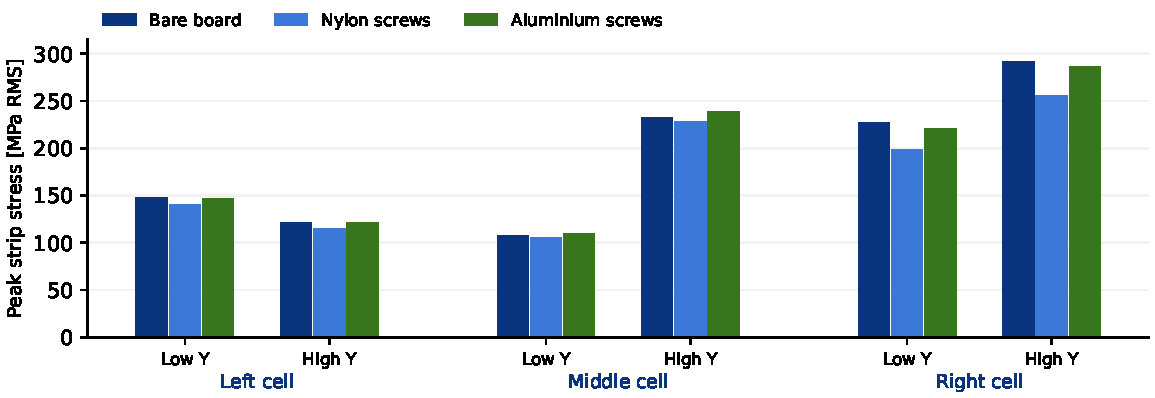
\includegraphics[width=.97\linewidth]{figures/raised-nickel-stress.pdf}
\captionof{figure}{Native one-sigma equivalent stress, maximized separately in each nickel strip. Low and high Y identify the strip ends near board coordinates 22 and 99~mm. Left, middle and right refer to increasing board X. For every strip, its maximum stayed at the same element corner across screw choices.}\end{center}

\heading{The assumed nickel yield stress is reached while the cells still clear the case}
The global model uses linear elastic nickel with modulus 220~GPa. The separate October nonlinear pull model assumes a 185~MPa initial yield stress for annealed nickel and a modulus of 205~GPa. To compare the two, we reconstructed the global \emph{signed} stress history during the first 0.1~s of the seeded October base-X waveform. At each sampled instant we added the six stress components from the locked preload to their respective dynamic components, then calculated von Mises stress at each corner. Independent spectral integration also reproduced all six native RMS component fields and the stored equivalent-stress field to within 0.0033\% relative field norm.

\begin{center}\small\begin{tabular}{lrrr}\toprule
First sampled crossing of 185 MPa & Bare & Raised / nylon & Raised / aluminium\\\midrule
Base X, time bracket [ms] & 38.116--38.132 & 38.956--38.971 & 38.116--38.132\\
Peak after tightening alone [MPa] & 161.9 & 162.1 & 162.1\\
Base X, minimum clearance bound [mm] & --- & 0.038 & 0.068\\\bottomrule\end{tabular}
\captionof{table}{Each time refers to this excitation with its prescribed 0.1~s ramp. The material threshold is a property assumed in the local model. Actual strip temper and weld properties would be needed to infer yielding or fatigue life.}\end{center}

The clearance check covers every quadratic exterior face on all three cells and the PLA. At the tightened position their separation exceeded 0.130~mm. We bounded the subsequent motion of each face by tracking its quadratic B\'ezier control points in a common translating frame at 65,536 samples/s. The two bodies' maximum excursions summed to 0.092~mm with nylon and 0.062~mm with aluminium through their respective threshold crossings. This places the early stress excursion before direct cell-to-case contact in both calculations. The air gap can close later in the same waveform (pages~10 and~15).

With base Z excitation, only the raised aluminium model crossed 185~MPa during the first 100~ms. The first crossing occurred at 77.911--77.927~ms on the middle cell attachment (STEP body~17). The same moving-surface bound gave at least 0.0256~mm of cell-to-case clearance through that sample. With base Y, all three models stayed below the reference throughout the 100~ms window.

\newpage
\pageheading{The local flush fixture exceeds the printed-PLA tensile references early in tightening}
The four outer washers first loaded the nylon-screw fixture at 0.59--0.63~mm of screw-head travel. Between 0.91 and 0.95~mm, the greatest tensile stress in the assumed print plane crossed 52.3~MPa. Through-layer tension crossed 40.5~MPa between 0.99 and 1.03~mm. These are typical tensile strengths for the 100\%-infill reference coupons. Comparing the native true stresses with these nominal coupon strengths gives an approximate check on the range of the elastic model. \href{https://wiki.polymaker.com/polymaker-products/more-about-our-products/documents/technical-data-sheets/pla/polylite-tm-pla}{Polymaker coupon data.}

\begin{center}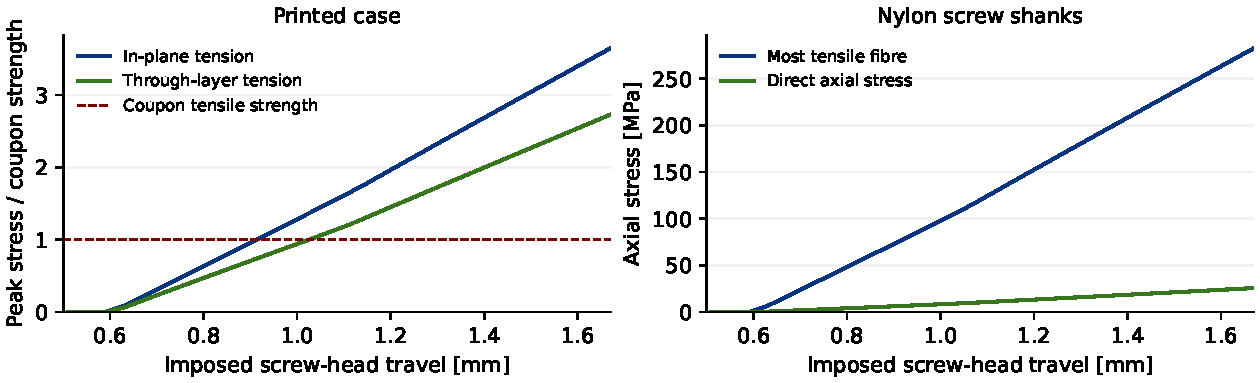
\includegraphics[width=.98\linewidth]{figures/flush-local-material.pdf}
\captionof{figure}{Native converged local states with rigid neighboring hardware and prescribed screw-head travel. Left, maximum tensile stress over the 16,108 quadratic PLA elements. Right, section-node tension including bending and the direct axial component in the four idealized short screw shanks. Curves stop at the last sampled travel before loaded penetration first exceeded 0.05~mm.}\end{center}

\begin{center}\small\begin{tabular}{lrr}\toprule
Local material reference & First corner crossing [mm] & First element with all four corners above [mm]\\\midrule
In-plane tension, 52.3 MPa & 0.91--0.95 & 1.55--1.59\\
Through-layer tension, 40.5 MPa & 0.99--1.03 & 2.57--2.61\\
Through-layer elongation, 1.8\% & 1.23--1.27 & No sampled element\\\bottomrule
\end{tabular}
\captionof{table}{The coupon elongation corresponds to logarithmic strain $\ln(1.018)=0.01784$. The first in-plane and through-layer stress crossings occurred 3.72 and 3.78~mm from the nearest coupled bearing node. Contact penetration already exceeded the local screen by the time all four corners of an element crossed the through-layer stress reference.}\end{center}

At 0.95~mm travel each prescribed screw head carried 64.0--64.5~N along board Z. The largest direct axial screw stress was 7.37~MPa. Including bending, the most tensile modelled screw fibre reached 85.34~MPa. A rigid connection between the screw rotation and its bearing footprint strongly influences that value. The McMaster-Carr listing for the representative nylon screw (93640A145) gives its dimensions and lists tensile strength as unrated. Its installed strength, head rocking and thread engagement therefore remain unverified. \href{https://www.mcmaster.com/products/nylon-allen-screws/}{McMaster-Carr screw data.}

\heading{How much moment each tab bearing carries}
At 0.91~mm of screw travel, before the first coupon crossing, the four local tab bearings carried 56.5--56.9~N each along board Z. For each bearing, we summed the axial nodal forces $F_{z,i}$ and their first moment about the screw axis. The equivalent offset $e=\|\sum_i {\bf r}_{xy,i}F_{z,i}\|/|\sum_i F_{z,i}|$ was 4.44--4.46~mm. Pressure acting in one direction inside a circular footprint of radius $R$ gives $e\leq R$. For the modeled $R=3.75$~mm, reproducing the observed moment using axial forces alone would require at least 5.2--5.4~N in the opposing direction per bearing. Forces from the printed solid and the screw/seat assembly agreed within 0.000003~N and moments within 0.00001~N~mm. An actual joint can also transfer moment through the shank, thread or head restraint.

For comparison, tightening the six original bolts in the raised full-board models produced a maximum case-screw fibre tension of 1.15~MPa with nylon and 1.63~MPa with aluminium. Neither raised case reached a printed-PLA coupon reference during tightening. The local flush trial subsequently crossed the board datum (page~11). Resolving the force required for an actual flush seat depends on the full-board contact path and the as-built material and joint behaviour.

\newpage
\pageheading{The left and centre cells reach the raised nylon case in the X movie}
The open-gap model puts the cell and PLA skins into intersection in frames 253--270 of the 480-frame X-axis movie. That is 4.20--4.48~s into playback, at 1.015442--1.016479~s in the load record. Checking all 1,917 integration samples in the clip identified two cells. The centre cell crossed first, then the left cell one sample later. The right cell stayed clear. All three stayed clear throughout the film interval for the other five mount and excitation combinations.

\begin{center}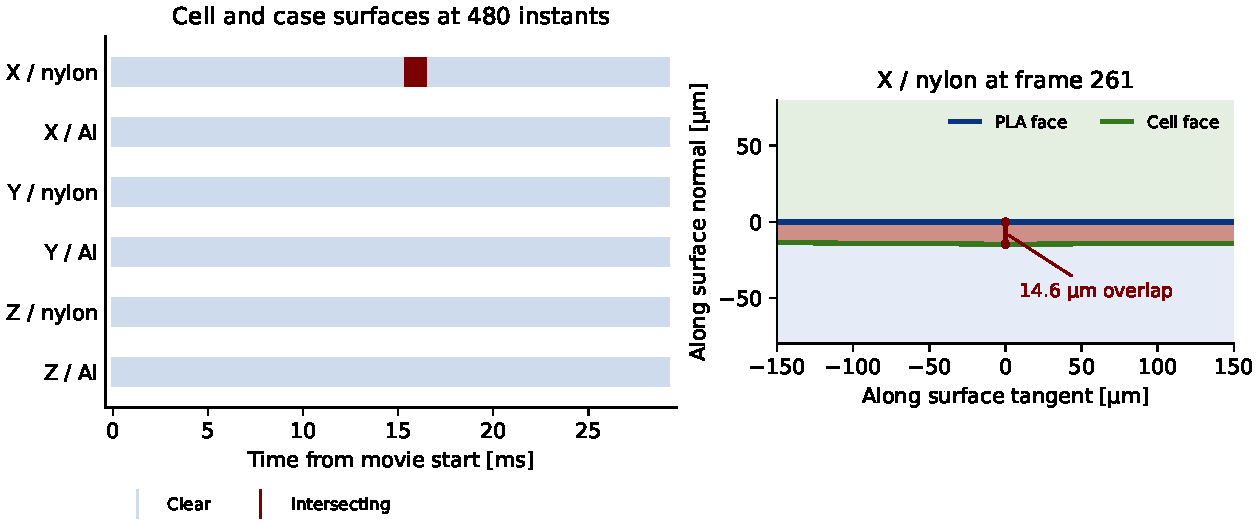
\includegraphics[width=.96\linewidth]{figures/raised-film-contact.pdf}
\captionof{figure}{Left, the cell and PLA surface check repeated at every displayed instant for each 3~mm mount and input axis. Right, the exterior surfaces at frame 262, cut in a plane through the closest PLA point and the most deeply embedded sampled cell vertex. Both section axes use the same scale.}\end{center}

\begin{center}\small
\begin{tabular}{lrrr}\toprule
Cell & Entry bracket [ms] & Exit bracket [ms] & Overlap at 15.869 ms [$\mu$m]\\\midrule
Left & 15.335--15.350 & 16.388--16.403 & 12.1\\
Centre & 15.320--15.335 & 16.418--16.434 & 11.3\\
Right & \multicolumn{2}{c}{Clear at all 1,917 samples} & ---\\\bottomrule
\end{tabular}
\captionof{table}{Physical time from the first movie sample. The $15.26~\mu$s integration step brackets entry and exit. Overlap is the sampled cell-vertex depth inside the curved PLA skin at one common instant. The nine-second MAPDL runs reproduced the independent surface classifications at all 1,917 movie-interval samples for both raised mounts and all three input axes.}\end{center}

At each mount's own peak dynamic PCB stress in the X clip, the smallest sampled cell-vertex gap was 0.149~mm at frame 228 for nylon and 0.146~mm at frame 290 for aluminium. The fixed-contact motion calculation omits any change in stress or trajectory caused by earlier contact.

\heading{Sensitivity to integration step and modal cutoff}
Independent integration displaced all 8,038 exterior quadratic PLA faces and all 938 cell faces. Subdividing their convex hulls established separation at clear samples. Two successive triangle refinements confirmed each crossing. The full closed skins gave 15.0~$\mu$m of sampled overlap with four segments per edge and 14.6~$\mu$m with eight at frame 262. The movie magnifies movement 50 times. The section above uses physical displacements.

For the nylon X history we halved and quartered the integration step, holding the piecewise-linear acceleration input fixed. Relative to the exact response of the modal oscillators to that input, the modal-coordinate differences fell from 0.401\% to 0.100\% and 0.025\%. All three time steps and the exact integration gave the same entry and exit brackets at the original sampling times. Retaining 35 modes through 2.95~kHz or 39 through 3.44~kHz gave the same brackets as the full 49-mode basis. Impact forces still require a contact-response calculation. \href{https://github.com/MDNich/MIT-RT-26_27-Work/blob/main/simulation_work/avionics/powerboardsim/2/output/videos/with_case/power_board_random_motion_4k60/random_fig06_baseX_responseX.mp4}{Raised cases under X-axis excitation.}

\newpage
\pageheading{The flush tabs make edge contact while most of each face stays open}
With nylon screws all four tabs first carried pressure between 2.60 and 2.675~mm travel. With aluminium all four were still clear at 2.90~mm and carried pressure at the final 3.00~mm equilibrium. Even there only 18.3--18.9\% of each aluminium-mounted tab lay within 0.05~mm of the board. The far sides retained 2.43--2.44~mm gaps. Both models exceeded the printed-PLA tensile references before tab contact. The resulting shapes describe an elastic continuation beyond the material data.

\begin{center}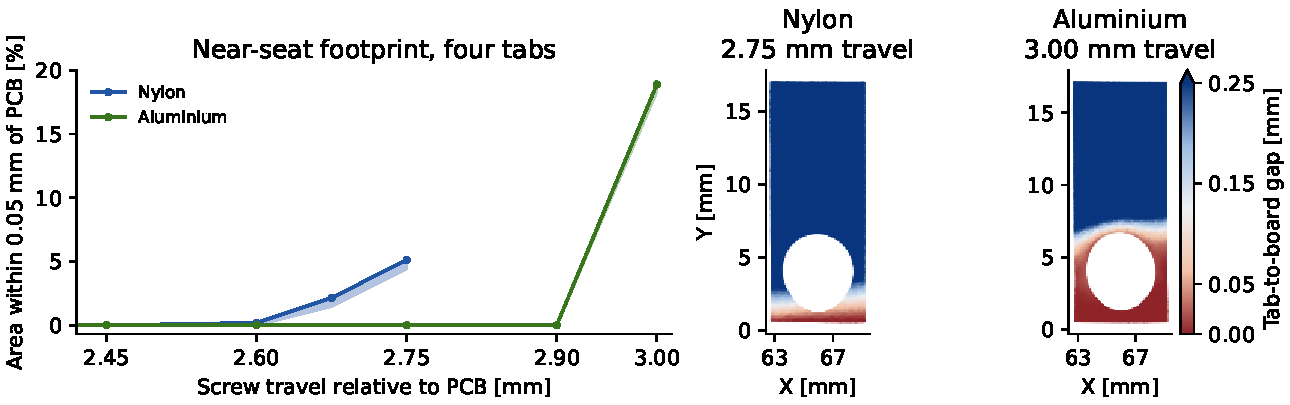
\includegraphics[width=.94\linewidth]{figures/flush-tab-seating.pdf}
\captionof{figure}{Near-seat area throughout the last increments. Lines mark the largest fraction among the four feet and shading spans their range. The maps show the high-X, low-Y tab at each trial's last equilibrium. White marks the bore, and the darkest blue denotes gaps of 0.25~mm or greater.}\end{center}

\begin{center}\small
\begin{tabular}{lrrr}\toprule
Tab position & Nylon near-seat area [\%] & Nylon largest gap [mm] & Al smallest gap [mm]\\\midrule
Low X, low Y & 4.4 & 2.425 & 0.218\\
Low X, high Y & 4.7 & 2.422 & 0.217\\
High X, low Y & 5.1 & 2.417 & 0.204\\
High X, high Y & 4.9 & 2.418 & 0.210\\\bottomrule
\end{tabular}
\captionof{table}{Near-seat area is the fraction of each overlapping tab footprint within 0.05~mm of the board. It was zero at every aluminium-mounted tab. All quantities are at 2.75~mm screw travel.}\end{center}

With nylon, the first through-layer tensile stress crossed 40.5~MPa between 0.95 and 1.10~mm, at a node tied to the idealized screw bearing. In-plane tension crossed 52.3~MPa at 1.10--1.25~mm. When the search excluded points within 2~mm of tied bearing nodes, both references were first crossed at 1.25--1.40~mm. The latter interval follows the first crossing of the 15~$\mu$m hardware-penetration screen (1.10--1.25~mm). At 2.75~mm the contact field reached 71~$\mu$m penetration. The nylon trial stopped at this equilibrium after three cutbacks. An installation-load rating requires measured print and contact behaviour.

The combined nylon result reproduced all 28 equilibria. The hardware contact audit included all 8,038 PLA contact faces. At 0.95~mm travel, before the first coupon crossing, the four original outer battery bolts gained 10.3--14.0~N above their 750~N locked preload. The two centre bolts changed by $-0.9$ and $+1.4$~N. At 0.95~mm the four drives supplied 25.59~mJ of work (28.41~mJ using alternate saved states). The PCB gained 8.81~mJ of stiffness energy, the PLA 8.01~mJ and the four screws 6.59~mJ. All element groups together accounted for 24.59~mJ.

\heading{Aluminium screws increase the load at the same drawdown}
In the two whole-board trials the screw shank geometry was identical. Only modulus, Poisson ratio and density differed between the decks. The first loaded hardware contact fell between 0.50 and 0.65~mm of relative travel for both mounts. At 0.80~mm, the four drives together carried 80.0~N with nylon and 115.6~N with aluminium. Peak through-layer PLA tension was 18.2 and 37.2~MPa respectively, against the 40.5~MPa coupon reference. With aluminium, both the in-plane and through-layer tensile references were first exceeded between 0.80 and 0.95~mm, while all four tab contacts remained open. In the 0.80~mm aluminium snapshot only the four outer washers intersected the PLA. Refining the curved surfaces gave up to 24.0~$\mu$m of sampled washer overlap, compared with 7.9~$\mu$m at loaded native contact corners. The smallest sampled cell clearance was 0.066~mm. At 3.00~mm travel, only the four outer washers intersected the PLA. Maximum sampled washer overlap was 0.136~mm and loaded native contact penetration was 0.109~mm, above the 0.015~mm screen. The three cells remained clear. A physically supported flush vibration state remains unresolved.

\newpage
\pageheading{The raised nylon case lowers the transverse load on all three cells}
Under base-X vibration, the X component of the right-hand cell's net dynamic force fell from 30.51~N RMS bare to 26.67~N with nylon screws and 29.73~N with aluminium. These are reductions of 12.6\% and 2.6\%. Nylon also reduced this load on the left and centre cells. Aluminium raised the centre-cell load from 25.60 to 26.28~N RMS. The PSD calculation keeps the tightened cell-to-case gap open. The two nickel attachments on each cell therefore carry its net dynamic load until additional contact occurs.

\begin{center}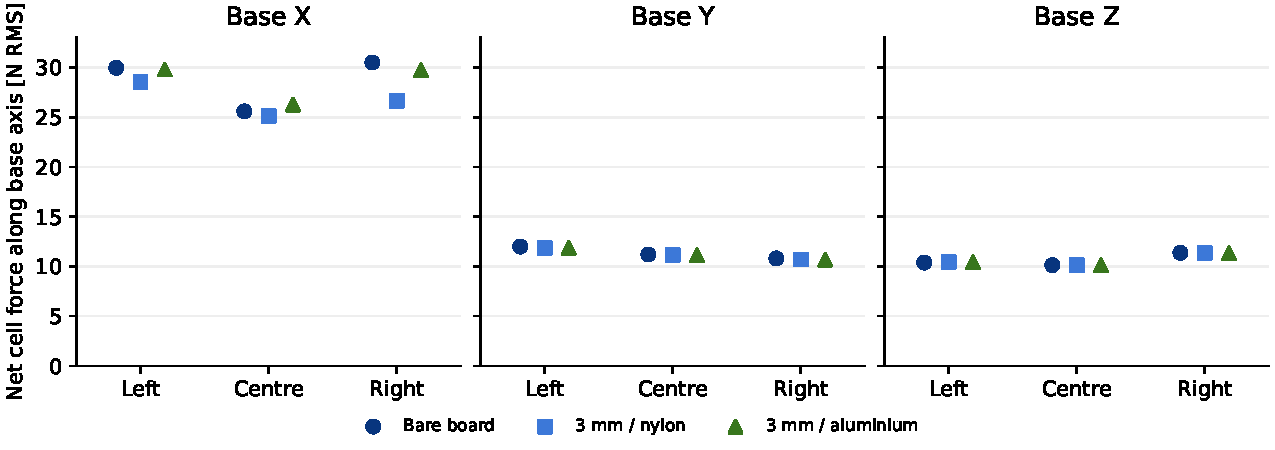
\includegraphics[width=.94\linewidth]{figures/raised-cell-inertial-force.pdf}
\captionof{figure}{Net force component parallel to each of three separate base excitations. Markers within each group correspond to the same physical cell. The ordinate is shared across panels. The material model gives each cell a mass of 55.38~g.}\end{center}

\begin{center}\small
\begin{tabular}{lrrr}\toprule
Base X, cell force [N RMS] & Bare board & 3 mm / nylon & 3 mm / aluminium\\\midrule
Left & 29.97 & 28.51 & 29.80\\
Centre & 25.60 & 25.13 & 26.28\\
Right & 30.51 & 26.67 & 29.73\\\bottomrule
\end{tabular}\end{center}

Along the excited direction, the Y and Z cases changed by less than 0.13~N on each cell. A transverse component can still grow. With Y input the X force on the left cell was 0.12~N RMS bare, 1.75~N with nylon and 1.01~N with aluminium. Page~22 compares the signed forces at both cell-to-nickel attachments.

\heading{Mass averaging and verification}
For each native mode we integrated the signed translations over each curved ten-node cell tetrahedron with its material density. The relative acceleration transfer function follows from differentiating modal displacement twice. We added the common base acceleration before integrating over the 20--2000~Hz spectrum. Combining the signed quantities in this order accounts for phase cancellation within the cell. Multiplying the resulting centre-of-mass acceleration by cell mass gives the force.

The four- and five-point-per-coordinate volume rules agreed within $10^{-9}$ in relative norm. Reducing the upper modal cutoff from 4 to 3.5~kHz changed the driven-axis forces by at most 0.30\%. Independent nodal acceleration RMS fields matched all nine native PSD fields within 0.044\% in relative norm over cell nodes. Separately, the original bare-board native time histories and original signed shapes reproduced the independently integrated seeded cell accelerations within 0.0075\%.

For the eight stationary seconds of the historical forcing, the driven-axis RMS loads differed from the continuous-spectrum estimates by at most 0.88\%. The largest discrepancy over all components was 10.4\% and occurred in a smaller transverse component. Evaluating the same sampled waveform with the discrete Newmark transfer function reproduced the time integration. At one-quarter of the historical time step, its largest discrepancy from the continuous-frequency response at the same Fourier bins fell to 0.59\%.

\newpage
\pageheading{The raised case preserves the first unpreloaded mode}
The first default-contact mode remained at 66.61~Hz for the bare board and both raised cases. The signed displacements of the 368,754 original solid nodes give a modal assurance criterion (MAC) above 0.999999 for both screw materials. The 20th modes tell a different story. Although each is the 20th frequency in its own assembly, the three shapes differ substantially.

\begin{center}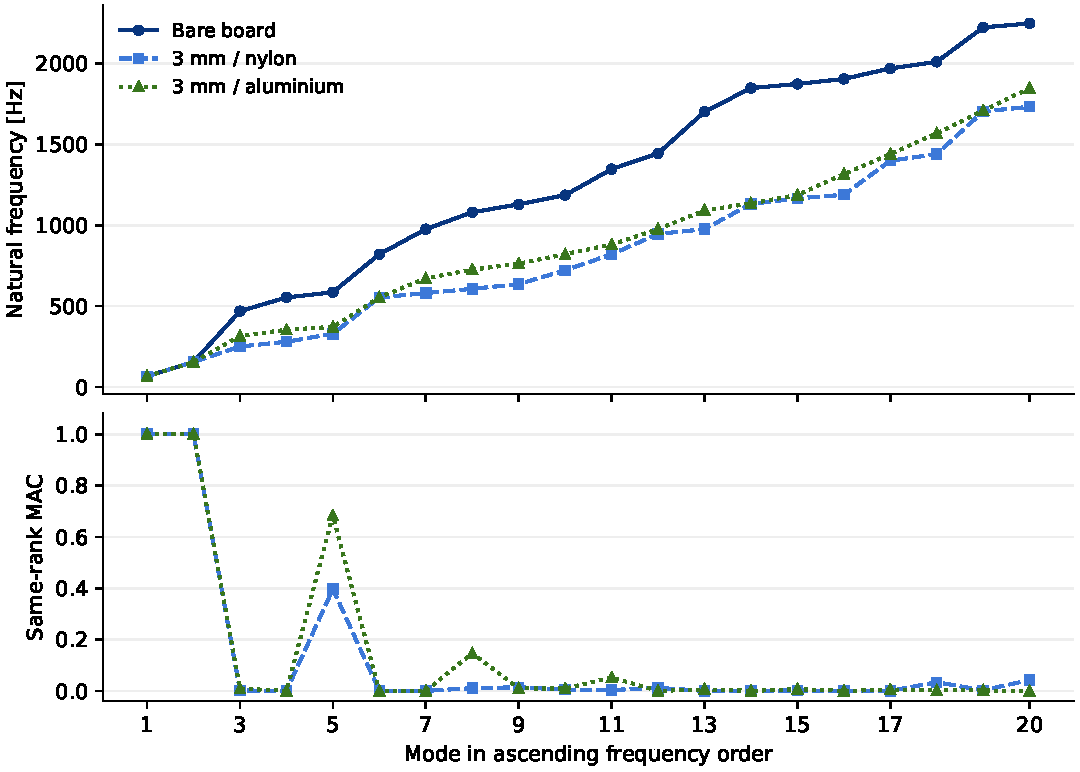
\includegraphics[width=.89\linewidth]{figures/default-mode-comparison.pdf}
\captionof{figure}{The upper panel orders each assembly's 20 native frequencies. The lower panel compares the bare and cased displacement vectors at equal rank. A value near one means that the original solid nodes moved in the same relative pattern.}\end{center}

\begin{center}\begin{tabular}{lrrr}\toprule
Mounting & Mode 1 [Hz] & Mode 20 [Hz] & Mode 20 MAC to bare\\\midrule
Bare &66.611 &2247.59 &1.000\\
3 mm, nylon screws &66.614 &1732.16 &0.042\\
3 mm, aluminium screws &66.615 &1847.75 &$<0.001$\\\bottomrule
\end{tabular}\end{center}
The closest shape to bare mode 20 within either raised set was mode 19. Even those correlations were weak (0.129 for nylon and 0.137 for aluminium). The displayed aluminium mode 20 instead matches bare mode 14 at 1847.75~Hz (MAC 1.000). A matching shape for bare mode 20 may lie above the extracted range.

\heading{Reading the mode movies}
Both default-contact movie pairs preserve the October mode ranks, a common colour range, and a 6~mm peak display amplitude. The raised panels identify the screw material, native frequency and shape correlation. These runs retain the original unpreloaded contacts. The tightened assembly has different equilibrium contact conditions and prestressed frequencies (page~8). Across the full catalogue, all 22 subjects now have a bare view and a comparison of both raised configurations. The flush assemblies still need an admissible installed state before their vibration fields can be shown.

\newpage
\pageheading{The two cell attachments carry opposing lengthwise forces}
The raised nylon case reduced the X force at both ends of all three cells under X excitation. Under Z excitation, however, both raised cases increased the force along the cell axis (Y) at all six attachments. The largest change occurred on the right-hand cell. The two ends carried 2.07 and 1.54~N RMS bare, 4.14 and 3.91~N with nylon screws, and 3.55 and 3.33~N with aluminium screws.

\begin{center}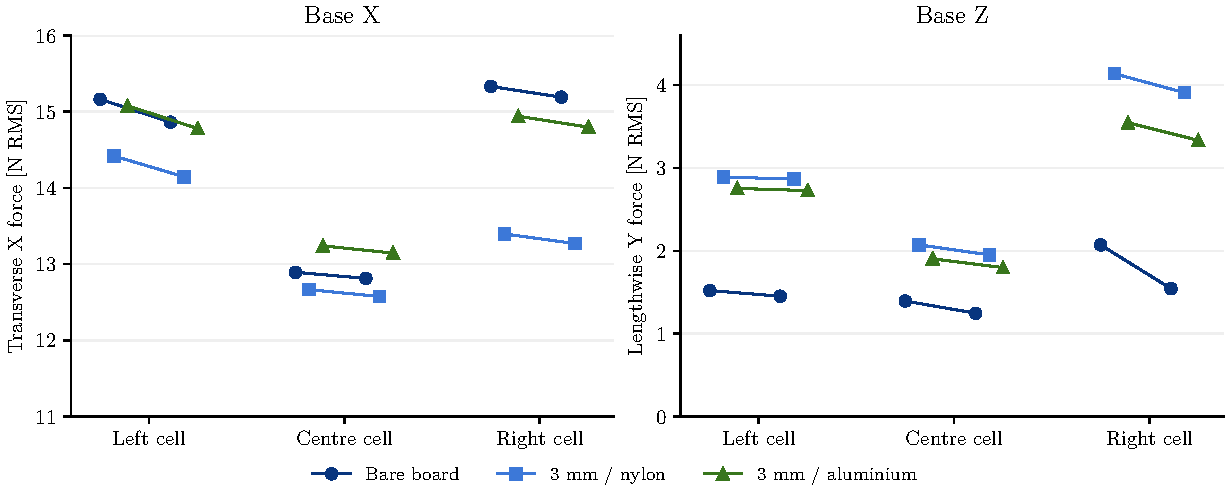
\includegraphics[width=.98\linewidth]{figures/cell-attachment-force.pdf}
\captionof{figure}{Each line joins the low-Y and high-Y ends of one cell. Left, the X force for base X. Right, the lengthwise Y force for base Z. Each marker gives the one-sigma force integrated over a complete cell-to-nickel attachment.}\end{center}

\heading{Why the whole-cell force can stay small}
For the right-hand cell under base Z, the two lengthwise force histories had correlations of $-0.88$ bare, $-0.97$ with nylon and $-0.97$ with aluminium in the spectrum calculation. When the signed forces were added before taking RMS, the corresponding net loads were only 1.03, 0.99 and 0.90~N. The opposing forces matter to the individual attachments even when they nearly cancel across the cell.

\begin{center}\begin{tabular}{lrrr}\toprule
Right cell, base X & Bare & Raised nylon & Raised aluminium\\\midrule
Low-Y end, X force [N RMS] &15.33&13.40&14.94\\
High-Y end, X force [N RMS] &15.19&13.27&14.80\\
Combined X force [N RMS] &30.52&26.66&29.73\\\bottomrule
\end{tabular}\end{center}

\heading{Force recovery and checks}
Both sides of each bond were identified from the native contact and target connectivity. For each tightened mode, the assembled solid-element stiffness and inertia forces cancel at free cell nodes. Summing the residuals on a bonded face gives its signed modal force. The adjacent nickel strip reproduced the opposite resultant to within 0.00032\% in vector norm for every mode. Independent frequency integration then combined the six bond resultants over the original base spectrum with 2\% modal damping.

For 90 sampled cell and nickel elements, the independently combined stiffness-force components agreed with all nine native PSD cases within 0.0056\% in relative norm. Under base X the summed X loads agreed with the whole-cell inertia calculation (page~20) within 0.42\%. Across Y and Z the corresponding differences reached 4.73\% and 2.16\%. Removing modes above 3.5~kHz changed any component by at most 0.362~N. The original October mode forces and native coordinates reproduced all 480 bare-board movie frames for all three drives within 0.00043~N per component.

The bonds cover the areas joined in the model. Actual weld sizes, local separation and the response after cell-to-case impact remain unmeasured.

\newpage
\pageheading{Case support shifts the peak dynamic load at the nickel attachments}
For each of the three original nine-second acceleration records, we recovered all three force components at both nickel attachments on each cell. We took the vector magnitude at each of the 589,825 saved instants, then found the largest magnitude across the six ends. These forces describe the extra load from vibration above the locked preload in the linear model.

\begin{center}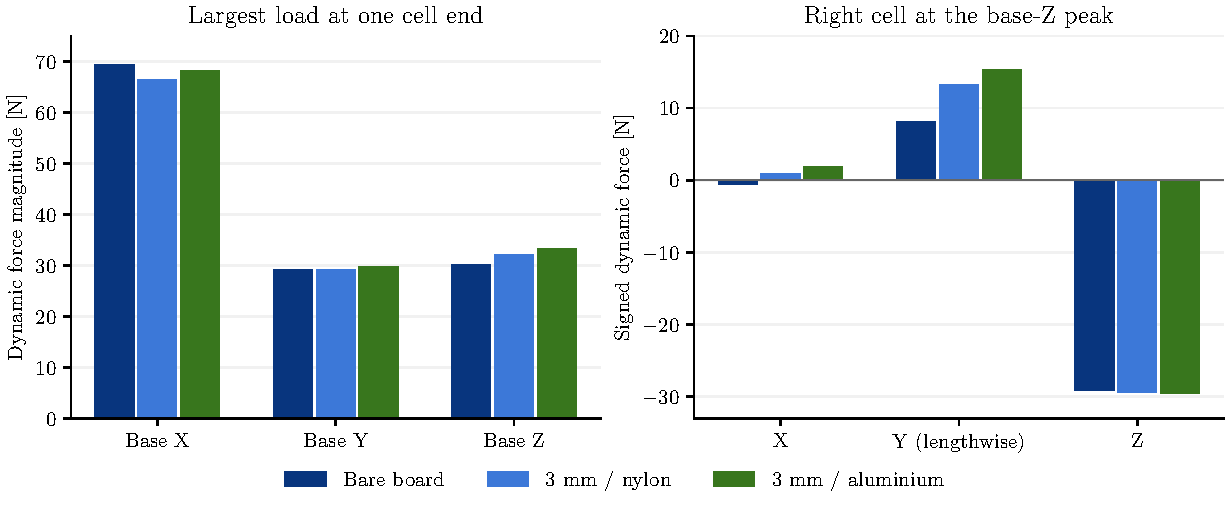
\includegraphics[width=.98\linewidth]{figures/attachment-native-history.pdf}
\captionof{figure}{Left, the maximum at a single cell end under each base direction. Right, the simultaneous signed components at the low-Y end of the right-hand cell. All three assemblies reached their base-Z maximum there at 1.86743~s. The positive lengthwise force increased with both raised mounts.}\end{center}

\begin{center}\small
\begin{tabular}{lrrrl}\toprule
Drive & Bare [N] & 3 mm nylon [N] & 3 mm aluminium [N] & Governing attachment\\\midrule
Base X & 69.39 & 66.39 & 68.23 & Left cell, low-Y end\\
Base Y & 29.25 & 29.17 & 29.79 & Left cell, end varies\\
Base Z & 30.22 & 32.21 & 33.30 & Right cell, low-Y end\\\bottomrule
\end{tabular}
\captionof{table}{Largest dynamic force magnitude at one cell-to-nickel bond over the full record. Under base Y the bare and nylon peaks occur at the high-Y end and the aluminium peak occurs at the low-Y end.}\end{center}

Under base X the peak end load fell by 4.3\% with nylon and 1.7\% with aluminium. Under base Z it rose by 6.6\% and 10.2\%. At the base-Z peak the Z component stayed close to $-29$~N in all three assemblies. The lengthwise component rose from 8.17~N bare to 13.21~N with nylon and 15.32~N with aluminium. The force on an individual attachment can therefore grow even while the two lengthwise end loads partly cancel across the cell (page~22).

\heading{Response before the nickel yield reference is reached}
The first 38.116~ms of base X precede the first sampled exceedance of the local pull model's 185~MPa nickel reference in any assembly (page~16). Over this common interval, the right cell's low-Y end carried the largest force in all three assemblies. Its magnitude reached 9.57~N bare, 8.92~N with nylon and 9.50~N with aluminium. The bounds on the raised assemblies' relative surface motion leave the cells clear of the PLA through this interval. The full-record peaks above include later excursions beyond the elastic and fixed-contact assumptions.

\heading{Numerical checks and physical scope}
The main results use signed native MAPDL time histories and bonded-interface forces from the prestressed modes. A separate integration of the same base motion reproduced the complete force fields within 0.002\% in relative norm. Restricting the modes to 3.5~kHz changed the nine peak magnitudes by at most 1.09\%. The bonded end area idealizes the battery-to-nickel attachment. The model supplies a dynamic resultant over that area. Predicting a weld failure load requires the actual weld geometry and material response.

\newpage
\pageheading{During startup, screw material changes which limit appears first}
In the raised aluminium mount under base X, tension across the assumed print layers reached the 40.5~MPa coupon mean at 63.54~ms. The first sampled cell-to-case intersection followed at 69.78~ms. With nylon screws the middle cell first intersected the case at 85.34~ms, while both PLA tensile stresses stayed below their respective coupon means throughout the 100~ms ramp. The nickel model had already exceeded its separate trial yield reference under X in all three assemblies (page~16).

\begin{center}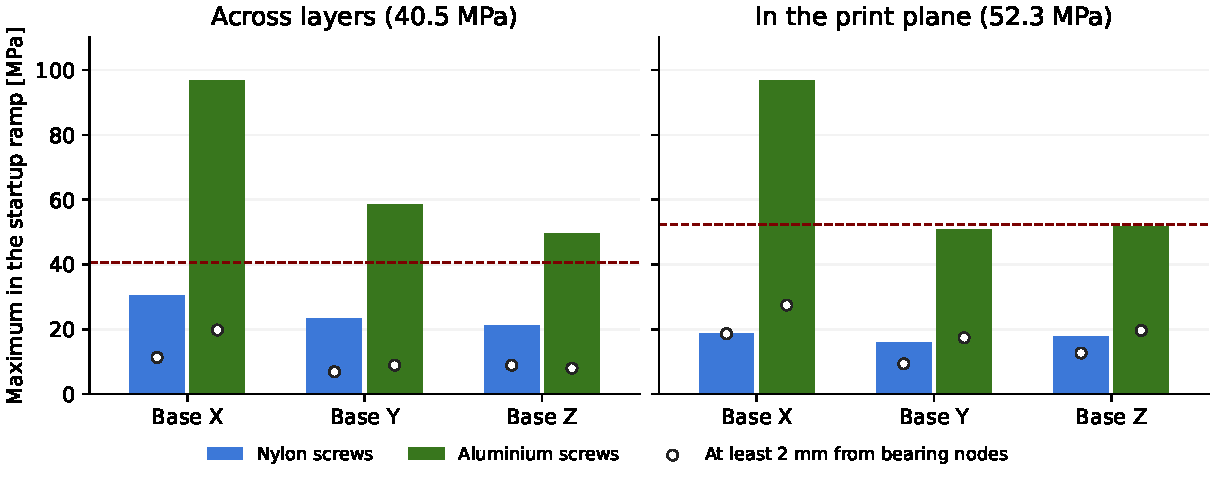
\includegraphics[width=.96\linewidth]{figures/startup-pla-stress.pdf}
\captionof{figure}{Peak tensile stress over 6,555 samples of each native waveform, including the locked preload. Bars include all 64,432 PLA element corners. White markers give the maxima among corners at least 2~mm from any node tied to a screw bearing. Dashed lines mark the coupon means.}\end{center}

\begin{center}\small
\begin{tabular}{llrrrr}\toprule
 & & \multicolumn{3}{c}{First sampled event [ms]} & Cell gap at layer\\
Screws & Base & Layer tension & In-plane tension & Cell intersection & crossing [mm]\\\midrule
Nylon & X & --- & --- & 85.34 & ---\\
Nylon & Y & --- & --- & --- & ---\\
Nylon & Z & --- & --- & --- & ---\\
Aluminium & X & 63.54 & 85.21 & 69.78 & 0.035\\
Aluminium & Y & 77.45 & --- & --- & 0.135\\
Aluminium & Z & 81.39 & --- & --- & 0.132\\\bottomrule
\end{tabular}
\captionof{table}{Times identify the first integration station meeting each criterion. The previous station was 15.26~$\mu$s earlier. Dashes in the three event columns mean the criterion was absent through 100.006~ms. Gap is the minimum sampled cell-vertex distance from the case across all three cells at the layer crossing.}\end{center}

The three aluminium layer crossings occurred within 0.54~mm of a node tied to a screw bearing. Outside the 2~mm band, both stresses remained below the coupon means for every input and screw material. On the aluminium X path, a cell surface was already inside the PLA when in-plane tension reached 52.3~MPa. The local bearing representation matters to the stress maximum. The comparison identifies where the fixed-contact, elastic calculation first reaches these particular screens. Failure of an actual printed tab depends on its print and bearing conditions.

\heading{Checks on the order of events}
Signed modal stresses were added to the locked stress tensor before evaluating layer-normal tension and the greatest in-plane principal stress. The search covered both screw mounts, all three base inputs and every stored station. The exact response of each modal oscillator to the piecewise-linear input reproduced the native tensile crossing brackets. Omitting modes above 3.5~kHz preserved those brackets and the first base-X cell crossing for both mounts. Independent integration shifted the first aluminium X intersection by one sample (15.26~$\mu$s) and reproduced the nylon onset. The cell check used the complete curved exterior surfaces. A separate intersection test at two surface refinements confirmed the cell states at the four aluminium tensile crossings.

\newpage
\pageheading{With nylon screws, the raised PLA case carries most of the pull at 0.50 mm}
The bare fixture and the raised fixture with nylon screws used the same nominal nickel damage law, 2,304 shell elements and two 750~N washer clamps. At a prescribed 0.500~mm of sideways travel, the bare edge cell required 11.33~N. The raised case required 141.82~N, of which the four case screws carried 112.62~N (79.4\%). At this displacement the neighbouring-cell support carried no net X load. The largest tensile stresses in the PLA were 28.75~MPa in the print plane and 23.60~MPa across the layers.

Local sliding at the washer--nickel interfaces began in the same 0.0500--0.0875~mm travel interval in both fixtures, before the cell touched the case. At 0.500~mm the peak element-averaged frictional stress rose from 0.801~MPa bare to 1.144~MPa cased, and peak accumulated tangential motion rose from 1.29 to 1.77~$\mu$m. Ten bare and eleven cased contact corners registered sliding. Every face with a sliding corner also retained a sticking corner.

\begin{center}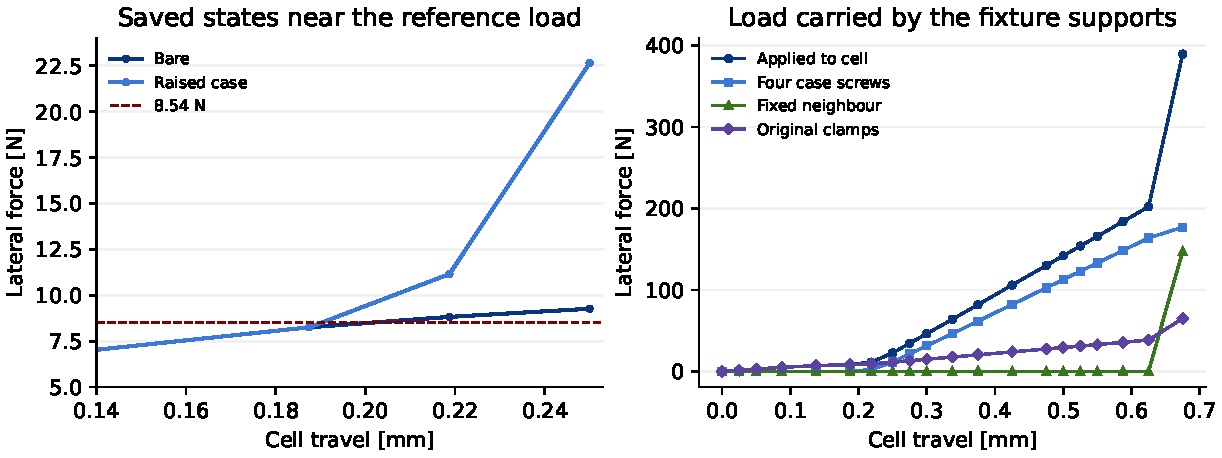
\includegraphics[width=.97\linewidth]{figures/stand3_nylon-damage-pull.pdf}
\captionof{figure}{Left, dashed lines join the original interval endpoints. The solid lines use 64 refined increments and coincide at 8.54~N. With nylon the native contact pair first carried load between 0.21191 and 0.21240~mm. Right, the load paths through the last station below the PLA and contact limits. The local fixture holds the other cells and the case screw tops fixed.}\end{center}

\begin{center}\small
\begin{tabular}{lrrr}\toprule
Nickel model & Bare travel at 8.54~N & Raised travel at 8.54~N & Force at 0.50~mm, bare / cased\\\midrule
Bilinear & 0.500~mm & 0.207~mm & 8.54 / 138.53~N\\
Multilinear with damage & 0.20190~mm & 0.20190~mm & 11.33 / 141.82~N\\\bottomrule
\end{tabular}
\captionof{table}{At 8.54205~N the refined bare, nylon and aluminium multilinear fixtures all gave 0.201904~mm between the same two saved stations. Both cases carried zero contact force there. At 0.212402~mm the first loaded face carried 0.114~N with nylon and 0.210~N with aluminium. The forces at 0.50~mm are saved equilibria for bare and nylon.}\end{center}

\heading{Printed-material scope and the last equilibrium}
The fixed neighbour began sharing the load between 0.625 and 0.675~mm of cell travel. At 0.675~mm the applied pull was 389.45~N. The case screws carried 176.89~N, the fixed neighbour carried 147.66~N and the original clamps carried 64.90~N. Between 0.675 and 0.725~mm the peak in-plane tension first exceeded the 52.3~MPa printed-coupon mean. The crossing occurred 4.36~mm from the nearest coupled bearing node. The first through-layer stress crossing followed at 0.800--0.825~mm. These local results depend on the actual stiffness of the mounts and neighbouring cells.

ANSYS retained 59 converged states, including 50 pull states, through 0.923275~mm. It terminated when the next increment failed to converge after cutbacks. None of the three nickel section summaries reached the $10^{-4}$ damage reporting threshold at any converged state. The two strips retained a graph path from the modelled battery attachment to the clamp at every station under the original October 0.99 section-damage diagnostic. The later equilibria extend beyond the onset of the printed-material limit. The contact-position comparison on page~5 also limits the interpretation of the low-load response. The physical rupture load remains unresolved.

\newpage
\pageheading{How the raised case changes strain in the nickel strips}
The three local fixtures used the same 2,304 nickel shell elements, multilinear plasticity and damage law, and 750~N washer preloads. In positive X, both original raised contact pairs first carried load between 0.1875 and 0.21875~mm. The STEP surfaces already intersected at the lower station (page~5). The last travel saved at exactly the same value in all three models before either raised fixture exceeded its material limits was 0.3375~mm.

\begin{center}\small
\begin{tabular}{lrrrr}\toprule
Fixture & Cell pull [N] & Case screws [N] & Strip clamps [N] & Peak nickel plastic strain\\\midrule
Bare & 10.15 & --- & 10.15 & 0.673\%\\
3~mm, nylon & 63.82 & 46.30 & 17.52 & 0.727\%\\
3~mm, aluminium & 125.98 & 100.18 & 25.81 & 0.783\%\\\bottomrule
\end{tabular}
\captionof{table}{Native reactions at 0.3375~mm. The fixed neighbour carried no lateral reaction at this travel. The maximum strain occurred in the same flat nickel shell element in all three models.}\end{center}

\begin{center}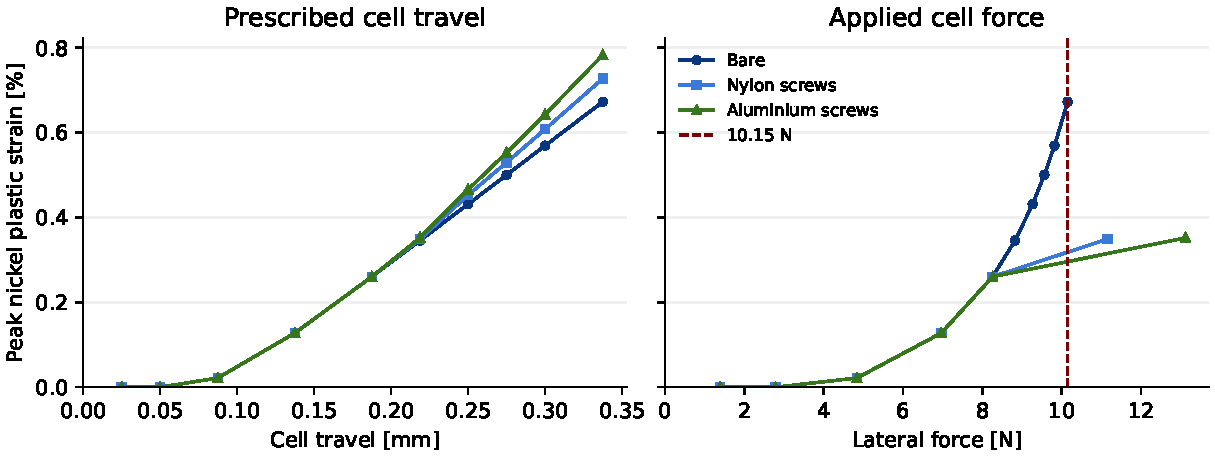
\includegraphics[width=.96\linewidth]{figures/raised-nickel-damage-strain.pdf}
\captionof{figure}{Each marker is a converged native state. The vertical line marks the 10.15~N reaction of the bare fixture at 0.3375~mm. Curves connect neighbouring states. Strain is the maximum element-averaged equivalent plastic strain across the three saved shell sections.}\end{center}

At equal travel, the aluminium fixture took almost twice the force of the nylon fixture. Both cased cells also strained the nickel more than the bare cell. At equal force, the comparison reverses. The cased stations bracketing 10.15~N had peak strains of 0.260--0.349\% with nylon screws and 0.260--0.352\% with aluminium, compared with 0.673\% at the bare station. The load bracket spans first contact in both cased fixtures. The difference between the screw materials at that force remains unresolved.

\heading{Where the aluminium result reaches its material limit}
At 0.425~mm the aluminium fixture carried 218.57~N, including 179.80~N through its four case screws. At the next saved equilibrium, 0.475~mm, in-plane PLA tension reached 60.16~MPa and through-layer tension reached 44.10~MPa. Both exceeded the printed-coupon means (52.3 and 40.5~MPa), within 0.54~mm of a tied screw-bearing node. With nylon screws the first tensile crossing occurred later, between 0.675 and 0.725~mm.

The aluminium solve retained 37 lateral equilibria through 0.87435~mm and stopped on the next increment. All 37 passed the original force-balance checks. The largest loaded-corner penetration was 0.0439~mm against the 0.05~mm local contact screen. Both nickel strips retained their modeled load paths and all three section damage summaries remained zero. The late equilibria exceed the PLA reference range, and the physical rupture load remains undetermined.


\heading{Nickel material-law check}
Three single-element tensile coupon reruns reproduced the October reaction, transverse displacement, axial stress, equivalent plastic strain and damage at all 1,074 shared stations. The peak reactions lay between 66.87 and 66.89~N. All three paths softened and stopped before the requested 1~mm extension. These numerical coupons verify the implemented material law. Predicting separation of the assembled strips also requires material and attachment measurements.


\newpage
\pageheading{How the vibration loads compare with component strength}
The high through-layer tension occurs in the \textbf{printed PLA tab beside the screw bearing}. The four case screws change how force enters the tab. For the assumed print, the manufacturer's tensile specimens reached a mean of 40.5~MPa across the layers and 52.3~MPa in the print plane. Each percentage below is the largest tensile stress in the stated record divided by its corresponding coupon mean. These ratios include bolt preload.

\begin{center}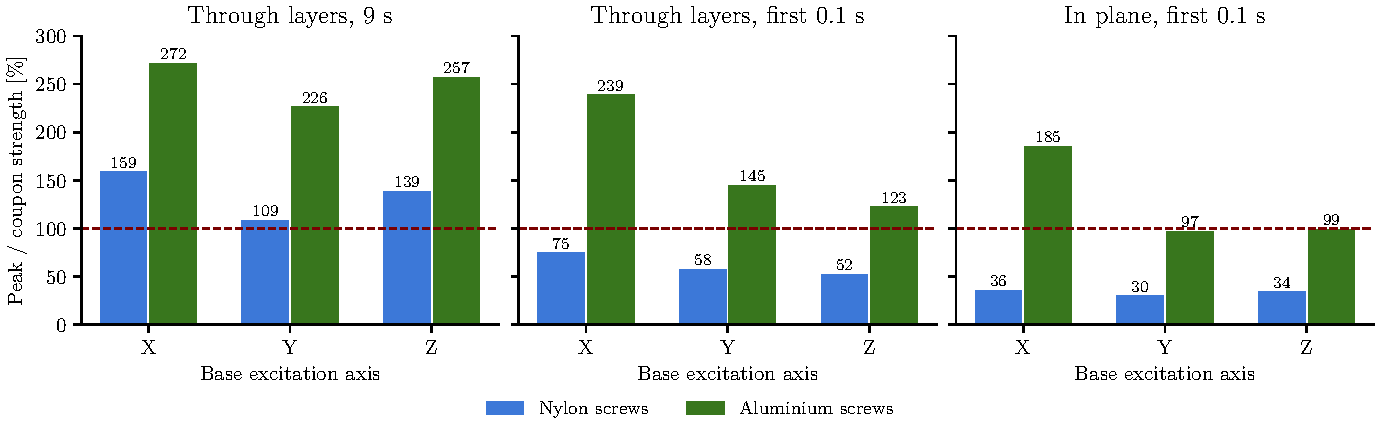
\includegraphics[width=.99\linewidth]{figures/pla-vibration-strength.pdf}
\captionof{figure}{Dashed lines mark 100\% of mean coupon strength. Left: peak signed through-layer stress at the bearing corner with the highest layer-normal RMS for each nine-second test. Centre and right: maxima over all PLA corners during the first 0.1~s. X, Y and Z were separate base excitations.}\end{center}

For board-normal vibration the monitored PLA tab reached 56.2~MPa with nylon screws and 104.2~MPa with aluminium screws. Both peaks occurred with the sampled cell and case skins clear at that instant. The linear model continues to store elastic stress beyond the coupon strength. At these peaks, actual load redistribution or cracking would require the print properties and screw-bearing compliance of the installed case. The earlier aluminium startup crossings occurred within 0.54~mm of a node tied to a screw bearing.

\heading{Other components}
\textbf{Nickel strips.} The nickel damage model assumes 185~MPa initial yield. Bolt tightening alone reached about 162~MPa (88\% of this reference). Under base X the signed, preload-inclusive stress crossed 185~MPa in all three assemblies within 39~ms (page~16). The actual temper and weld geometry are needed to assess strip rupture or fatigue life.\\
\textbf{Board and soldered parts.} Board-normal base vibration produced 32.5, 64.8 and 84.2~MPa RMS in the equivalent PCB material for bare, nylon and aluminium, respectively. These statistical stresses show how the board response changes. A strength margin for a populated assembly requires the actual laminate allowables and package-specific limits on local board strain or solder fatigue.\\
\textbf{Case screws and cell attachments.} At 0.3375~mm lateral travel the modeled peak tensile screw-fibre stresses were 13.1~MPa (nylon) and 34.2~MPa (aluminium). The nylon reference screw has no rated tensile strength in its listing, and the aluminium alloy and temper are unspecified. The attachment calculations give force over the idealized bonded footprint. A tested weld strength is needed to turn that force into a margin.

{\small \href{https://wiki.polymaker.com/polymaker-products/more-about-our-products/documents/technical-data-sheets/pla/polylite-tm-pla}{Printed PLA tensile data}\quad|\quad\href{https://www.electronics.org/TOC/IPC-9704A.pdf}{IPC/JEDEC guidance on measuring board strain near components}}


\newpage
\pageheading{A 2.5 mm stand-off leaves clearance at the lips and under the cells}
For the supplied Balius STEP at its nominal hole alignment, four outer washers set the closest rigid mounting position. They first touch at a 2.397~mm tab-to-PCB spacing. At 2.500~mm they clear by 0.103~mm. The cells approach the sides of their circular pockets much more closely than the floors.

\begin{center}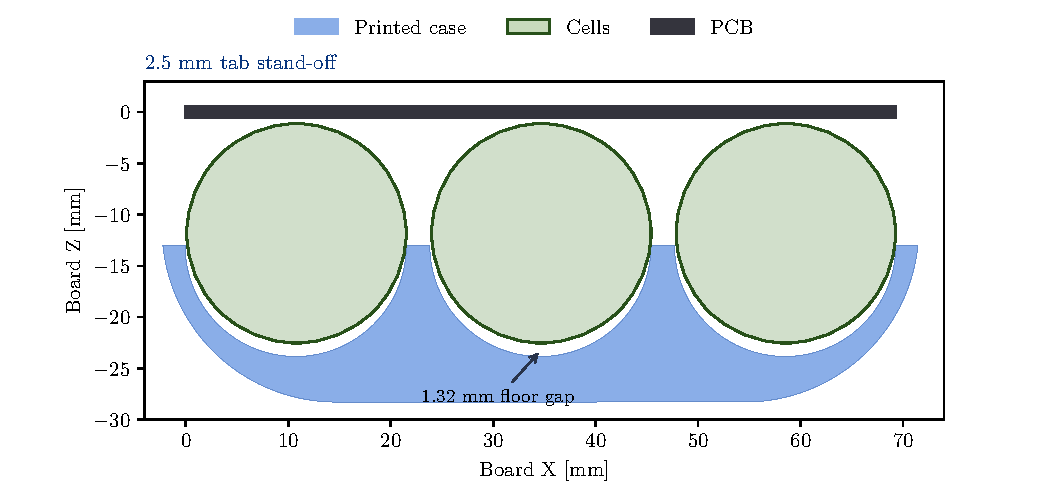
\includegraphics[width=.99\linewidth]{figures/midspan-fit-2p5mm.pdf}
\captionof{figure}{Section at the case midspan using the STEP profile and 10.700~mm cell radii. The 1.32~mm dimension is vertical beneath the middle cell. Washers and mounting tabs sit outside this plane. The drawing uses the same scale for both axes.}\end{center}

\begin{center}\small\begin{tabular}{lrrr}\toprule
Tab-to-PCB spacing & Left cell minimum & Middle cell minimum & Right cell minimum\\\midrule
2.400~mm & 0.082~mm & 0.065~mm & 0.082~mm\\
2.500~mm & 0.093~mm & 0.076~mm & 0.093~mm\\
3.000~mm & 0.161~mm & 0.144~mm & 0.161~mm\\\bottomrule
\end{tabular}
\captionof*{table}{Shortest three-dimensional surface distances between each undeformed cell and the case. The 2.400~mm setting leaves just 0.003~mm between the case and the first four washers.}\end{center}

Holding the board and cells fixed, the middle cell would first touch as spacing fell to about 1.240~mm, then the outer cells near 1.210~mm. Reaching either position requires interference with the existing washers. A 2.5~mm spacer can therefore give a close nominal side fit, while simultaneous supported contact of all three rigid cells requires a change to the installation geometry or compliance. Actual print dimensions, washer stack and cell positions determine the as-built clearances.


\newpage
\pageheading{Which battery case fits the archived board?}
The Balius SolidWorks part gives the closest nominal fit of the three files examined. The supplied Balius STEP and the fresh native export share the same three cell-pocket axes and radii. The native part provides additional space around the washers. SolidWorks 2026 SP4.1 exported the default configuration of each native part to AP203 STEP with zero reported errors or warnings. Each export reopened as one solid.

\begin{center}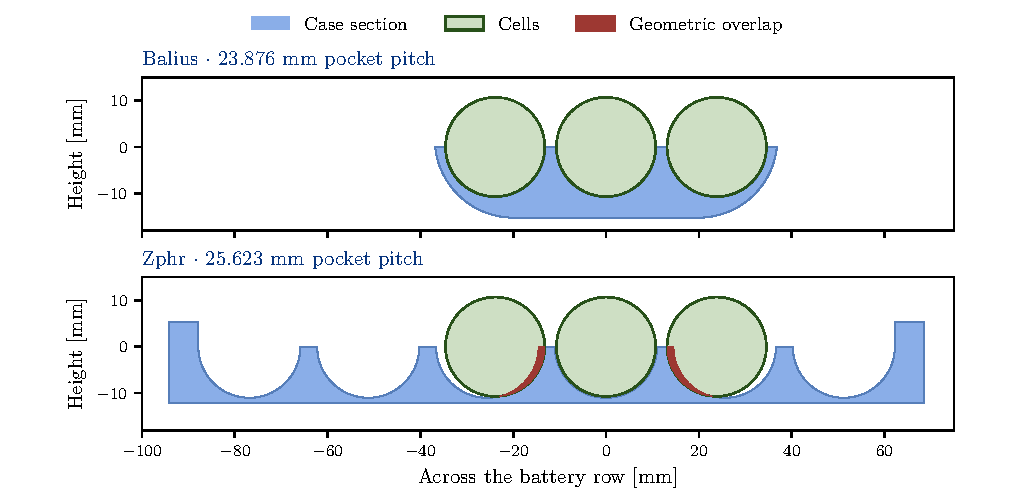
\includegraphics[width=.98\linewidth]{figures/alternate-case-sections.pdf}
\captionof{figure}{Midspan sections at equal scale. For this pocket comparison, the middle cell axis coincides with one pocket axis in each direction. Red marks where the outer cells intersect the Zphr case in this pose. The mounting holes are checked separately.}\end{center}

\heading{Balius at 1.25 mm tab-to-board spacing}
A rigid sweep over the 35 archived hardware solids found that the native part reaches the middle cell first at 1.240~mm stand-off. The outer cells reach their pockets at 1.210~mm if the geometry is allowed to continue through first contact. The earliest outer-washer contact in that continuation is at 0.733~mm. With the original supplied STEP, the washers touch at 2.397~mm, before any cell can reach its pocket.

\begin{center}\small\begin{tabular}{lrrr}\toprule
Case and tab spacing & Middle cell gap & Outer cell gaps & Smallest outer-washer gap\\\midrule
Supplied Balius STEP, 2.50 mm & 0.076 mm & 0.093 mm & 0.103 mm\\
Balius native export, 2.50 mm & 0.076 mm & 0.093 mm & 1.250 mm\\
Balius native export, 1.25 mm & 0.003 mm & 0.020 mm & 0.328 mm\\\bottomrule
\end{tabular}\end{center}
At 1.25~mm all three cells sit close to the native pockets. The small clearances depend on the actual print, battery sleeves, washer stack and board alignment. The reported structural and vibration results use the originally supplied STEP.

\heading{Zphr pocket and screw alignment}
Zphr has six pockets of radius 11.000~mm and pitch 25.623~mm. The three 10.700~mm-radius cells have adjacent pitches of 23.893 and 23.859~mm. Centring the middle cell in a Zphr pocket puts the outer cell axes 1.729 and 1.764~mm off-centre in the neighbouring pockets. The available concentric radial clearance is only 0.300~mm.

The 14 Zphr bores have 3.400~mm through diameter. Comparing inter-hole distances over every assignment of four bores to the board corners proves that at least one centre is displaced by at least 10.525~mm under any rigid planar alignment. A nominal M3 screw can accommodate only 0.800~mm of centre offset across the case and PCB bores. Changing stand-off alone cannot register this pattern.

\newpage
\pageheading{The raised case engages later when the pull reverses}
We pulled the same outer cell in both directions along PCB X. For each mounting configuration, the two solved input decks had the same geometry, clamp preload, bilinear nickel law and load increments. The only numerical change was the sign of the prescribed cell travel. Each native result contains 33 converged equilibria.

\begin{center}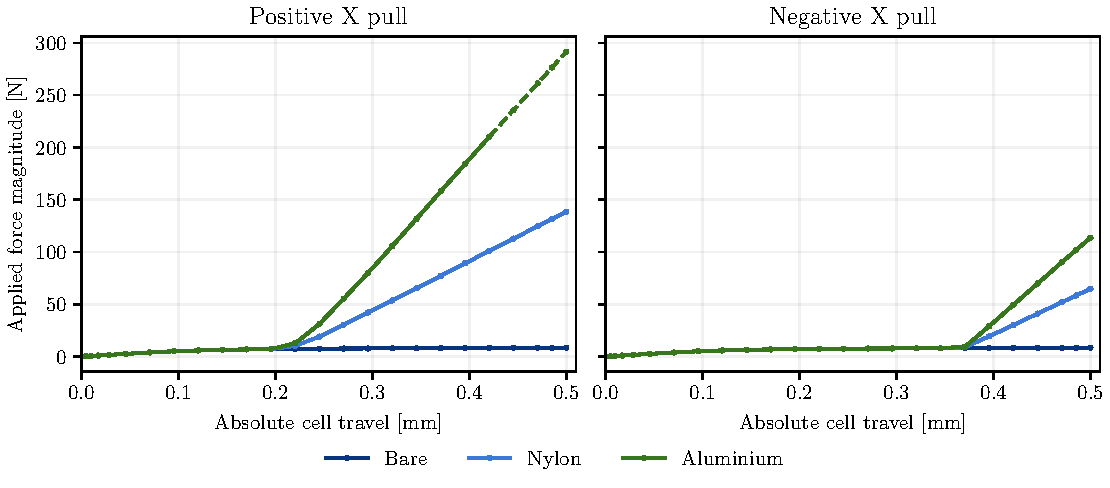
\includegraphics[width=.98\linewidth]{figures/directional-pull.pdf}
\captionof{figure}{Applied cell force at equal travel magnitudes for the bare board and the two 3~mm mounts. Dashed segments follow the linear PLA model beyond its first printed-material reference. All six curves use the October bilinear nickel law. The multilinear nickel results are on pages~25--26.}\end{center}

\heading{Force at a common displacement}
At 0.420625~mm, all six fixtures remained within the printed-material and contact-penetration screens where applicable. The bare forces in opposite directions differed by only 0.027~N. Reversing the pull reduced force by 70\% with nylon case screws and 76\% with aluminium screws.

\begin{center}\small\begin{tabular}{lrrrr}\toprule
 & \multicolumn{2}{c}{Applied cell force [N]} & \multicolumn{2}{c}{Via four case screws [N]}\\
Mount & $+X$ & $-X$ & $+X$ & $-X$\\\midrule
Bare & 8.26 & 8.24 & --- & ---\\
Nylon & 100.99 & 30.17 & 80.00 & 18.91\\
Aluminium & 209.96 & 49.42 & 174.54 & 35.58\\
\bottomrule\end{tabular}
\captionof*{table}{Force magnitudes at 0.420625~mm of cell travel. Each value comes from a saved native equilibrium. The original nickel clamps carry the remainder in these fixtures.}\end{center}

\heading{Clearance and first load}
Under a pure X translation of the undeformed STEP cell, the gap first closes after 0.163~mm toward positive X and 0.308~mm toward negative X. In the native fixtures the cell can also rotate. The moving-cell contact pair first registered closure between 0.196--0.221~mm in positive X and 0.346--0.371~mm in negative X for both screw materials. The later engagement leaves less reverse travel over which the case can take load.

At 0.500~mm in negative X, the applied force was 8.51, 64.73 and 113.46~N for the bare board, nylon and aluminium respectively. The corresponding maximum nickel plastic strains were 1.252, 1.346 and 1.434\%. Peak in-plane PLA tension at that reverse endpoint reached 23.58~MPa with nylon and 43.07~MPa with aluminium (45\% and 82\% of the 52.3~MPa coupon mean). Both reverse paths stayed within the recorded contact and PLA screens. The fixed screw tops represent a local fixture. These loads describe a prescribed displacement and do not establish a rupture load.

\end{document}
